\documentclass[a4paper]{report}
\usepackage[utf8]{inputenc}
\usepackage[spanish]{babel}
\usepackage[dvipsnames]{xcolor}
\usepackage{parskip}
\usepackage[colorlinks=true,urlcolor=blue,linkcolor=black]{hyperref}
\usepackage{url}
\usepackage{float}
\usepackage{amsmath,amssymb}
\usepackage{graphicx}
\usepackage{geometry}
\usepackage{caption}
\usepackage{wrapfig}
\usepackage{fancyvrb}
\usepackage{lmodern}
\usepackage{color,array}
\usepackage{etoolbox}
\usepackage{minted}
\usepackage{xpatch}
\usepackage{subfig}
\usepackage{colortbl}
\usepackage{tikz}
\usetikzlibrary{calc,tikzmark,arrows}
\usepackage{svg}
\usepackage{color,soul}
\usepackage{tcolorbox}

% mips-lexer.py HAS TO HAVE execution permissions for this to work
% minted uses which to detect the file:
% https://github.com/gpoore/minted/blob/d46f1ba2d248f2f3504bcc795dd39c613bd3c5a0/source/minted.sty#L197
\renewcommand{\MintedPygmentize}{./mips-lexer.py}

\makeatletter
\patchcmd{\@makechapterhead}{\vspace*{50\p@}}{}{}{}% Removes space above \chapter head
\patchcmd{\@makeschapterhead}{\vspace*{50\p@}}{}{}{}% Removes space above \chapter* head
\makeatother

\xpretocmd{\chapter}{\setcounter{section}{0}}{}{}

\makeatletter
\newcount\my@repeat@count
\newcommand{\myrepeat}[2]{%
    \begingroup
    \my@repeat@count=\z@
    \@whilenum\my@repeat@count<#1\do{#2\advance\my@repeat@count\@ne}%
    \endgroup
}
\makeatother

\unaccentedoperators

\definecolor{autumn-red-pyg}{HTML}{AA0000}
\definecolor{autumn-blue-pyg}{HTML}{0000AA}
\definecolor{autumn-gray-pyg}{HTML}{AAAAAA}
\definecolor{autumn-teal-pyg}{HTML}{00AAAA}
\definecolor{murphy-green-pyg}{HTML}{008000}
\definecolor{murphy-periwinkle-pyg}{HTML}{ABABFF}
\definecolor{murphy-deepsea-pyg}{HTML}{005487}

\setlength{\textfloatsep}{0pt}
\counterwithout{section}{chapter}
\usemintedstyle{default}

\title{\Huge{}\texttt{MIPS R2000}\\\vspace{8pt}\Large{}\textbf{\scalebox{.85}[1.0]{Práctica 1}}}
\author{Ariel Leonardo Fideleff}

\begin{document}

\pagenumbering{gobble}
\maketitle

\chapter{Cuestiones}

\section{Apartado 1}

\begin{center}
\large\textbf{-- \textsl{Declaración de palabras en memoria} --}
\end{center}

\subsection*{1.1 y 1.2}

Como podemos ver en la Figura \ref{fig:c1-1}, los dos números enteros reservados en el programa se ubicaron en las posiciones \texttt{0x10010000} y \texttt{0x10010004}, distanciados justamente por 4 bytes ya que se corresponde con el tamaño de palabra. Es decir, si cada entero fue reservado como un \mintinline{mips}{.word}, cada uno ocupa 4 bytes. Con esto, sumado a que el ensamblador los coloca uno seguido del otro en la memoria, dado que el primer valor por defecto comienza en la posición \texttt{0x10010000}, el segundo necesariamente deberá ubicarse 4 posiciones de memoria después (cada posición se corresponde con un byte).

En cuanto a los valores como tal, podemos ver la diferencia en que hayamos indicado uno en decimal, mientras el otro en hexadecimal. De esta forma, el número 15 en decimal es representado como \texttt{0x0000000f} en hexa, forma con la cual se presenta en el panel de datos. Mientras, el segundo valor, al haber sido especificado en el programa en base 16, lo reconocemos fácilmente como \texttt{0x00000015} en el panel en cuestión.

\begin{figure}[h]
    \centering
    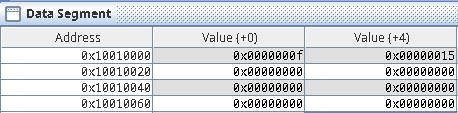
\includegraphics[width=.7\linewidth]{img/c1-1}
    \caption{Datos del programa según se indican en el panel de datos}
    \label{fig:c1-1}
\end{figure}

\subsection*{1.3}

De acuerdo a lo dicho en la teoría, las etiquetas \texttt{palabra1} y \texttt{palabra2} deberían tomar el valor de las posiciones de memoria a las que hacen referencia. En este caso, las ya mencionadas \texttt{0x10010000} y \texttt{0x10010004}, respectivamente.

De hecho, como se muestra en la Fig. \ref{fig:labels-fst}, esto lo podemos comprobar en la ventana \textit{Labels}, que se puede activar desde la configuración del simulador.

\begin{figure}[h]
    \centering
    \captionsetup{justification = centering}
    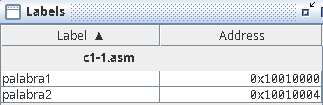
\includegraphics[width=.5\linewidth]{img/c1-3}
    \caption{Valores de las etiquetas \texttt{palabra1} y \texttt{palabra2} en la ventana \textit{Labels}}
    \label{fig:labels-fst}
\end{figure}

\subsection*{1.4}

Al ensamblar el programa dado, no parece presentar ninguna diferencia con respecto al primer programa visto, ya sea tanto en la memoria, como también en otras variables visibles en el simulador (por ejemplo, los registros).

\subsection*{1.5}

El siguiente código cumple con la consigna planteada:

\vspace{7pt}
\inputminted[linenos]{mips}{src/cuestiones/c1-5.asm}
\vspace{7pt}

Y en la Figura \ref{fig:arr5-mem} podemos comprobar que los valores fueron almacenados de forma correcta, considerando que los números 30 y 60 en decimal se corresponden con \texttt{0x0000001e} y \texttt{0x0000003c} en hexadecimal, respectivamente.

\begin{figure}[h]
    \centering
    \captionsetup{justification = centering}
    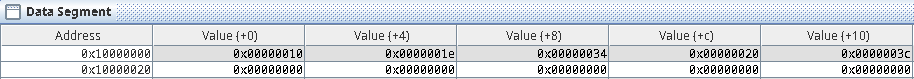
\includegraphics[width=.95\linewidth]{img/c1-5a}
    \caption{Valores del vector de números declarado en el programa propuesto, según se indican en el panel de datos}
    \label{fig:arr5-mem}
\end{figure}

Notar que al haber cambiado la dirección de memoria inicial donde se quiere que se almacenen los datos (respecto a la utilizada por defecto), debimos de expandir el panel de datos del simulador para poder visualizar el segmento de la memoria donde se ubicaban los valores reservados de nuestro vector, seleccionando la opción correspondiente desde un menú desplegable, tal como se lo muestra en la Figura \ref{fig:dropdown-data}.


\begin{figure}[h]
    \centering
    \captionsetup{justification = centering}
    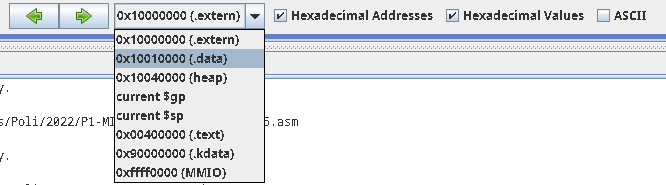
\includegraphics[width=.7\linewidth]{img/c1-5b}
    \caption{Menú desplegable para seleccionar la visualización del segmento de memoria correspondiente al utilizado por el programa planteado}
    \label{fig:dropdown-data}
\end{figure}

\subsection*{1.6}
\label{sec:c1-6}

Podemos probar cambiar el argumento de la directiva \mintinline{mips}{.data} para intentar almacenar los datos partiendo desde la dirección \texttt{0x10000002}:

\vspace{7pt}
\inputminted[linenos]{mips}{src/cuestiones/c1-6.asm}
\vspace{7pt}

Hecho este cambio, el panel de datos nos muestra que los valores ahora son almacenados partiendo desde la dirección de memoria \texttt{0x10000004}, saltando de 4 en 4 (por el tamaño de palabra, Fig. \ref{fig:not-multiple}).

\begin{figure}[h]
    \centering
    \captionsetup{justification = centering}
    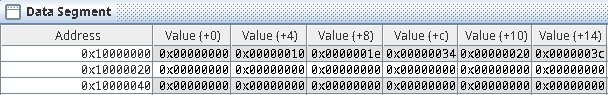
\includegraphics[width=.8\linewidth]{img/c1-6}
    \caption{Valores y respectivas posiciones de memoria del programa con argumento de \mintinline{mips}{.data} modificado}
    \label{fig:not-multiple}
\end{figure}

Esto difiere en principio de lo que uno podría esperar, ya que se le está indicando al ensamblador que ubique la información partiendo desde la dirección de memoria \texttt{0x10000002}. El motivo por el cual ejecuta el cambio descripto, es porque se requiere que la ubicación de todos los valores se encuentren en posiciones múltiplos de 4, de forma que la memoria ``esté alineada''. Éste es un requisito de la arquitectura MIPS, o bueno, al menos estamos seguros basándonos en lo visto en la teoría, que lo es para el lenguaje de máquina de los microprocesadores MIPS R2000.

Con esto en cuenta, el ensamblador, sabiendo que indicamos el espacio para datos partiendo desde la posición de memoria \texttt{0x10000002}, buscó por la posición de memoria (mayor o igual) múltiplo de 4 más cercana, y a partir de allí ubicó los valores del vector de números reservado en el programa.

\begin{center}
\large\textbf{-- \textsl{Declaración de bytes en memoria} --}
\label{sec:decl-byte-mem}
\end{center}

\subsection*{1.7 y 1.8}

\begin{wrapfigure}[11]{r}{.25\linewidth}
    \centering
    \captionsetup{justification = centering}
    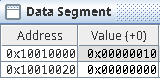
\includegraphics[width=\linewidth]{img/c1-7}
    \caption{Representación del contenido especificado en la memoria, visto desde el panel de datos}
    \label{fig:c1-7}
\end{wrapfigure}

Como ya sabemos, al no especificar ningún argumento para la directiva \mintinline{mips}{.data}, los datos se ubicarán partiendo desde la dirección de memoria \texttt{0x10010000} por defecto.

Además, al tratarse de un único byte, y considerando que el valor indicado \texttt{0x10} no supera el tamaño permitido por la directiva (el máximo valor posible sería \texttt{0xFF}), éste se almacenaría ``al comienzo de la palabra'', efectivamente implicando que el valor de la palabra que contiene el byte sea el mismo al especificado. Al fin y al cabo, el tamaño de una palabra es mayor al de un byte (justamente, 4 bytes), por lo que resulta en que el valor de la palabra sea el mismo al valor del tamaño de un byte, antecedido por 0s que no cambian el entero final almacenado.

\subsection*{1.9 y 1.10}
\label{sec:c1-10}

En este caso, se almacenan los valores \textbf{\texttt{0x40302010}} y \textbf{\texttt{0x10203040}} en las posiciones de memoria \textbf{\texttt{0x10010000}} y \textbf{\texttt{0x10010004}} respectivamente.

Si bien el segundo valor es indicado como tal de forma explícita en el código presentado, el primer valor, en cambio, es el resultado de almacenar un vector de 4 valores especificados del tamaño de 1 byte. Esto nos muestra que el simulador, por un lado, almacena los valores indicados con la directiva \mintinline{mips}{.byte} de forma contigua, independientemente de que los valores sean accedidos de a una palabra a la vez. Por otro lado, nos indica también el orden que utiliza para guardar los datos dentro de una palabra, el cual puede ser identificado afín con el concepto de \textit{Little-Endian}, el cual consiste en la organización y alineamiento de los datos de forma que, aplicado a este caso, ``lo que va primero'' se almacene en las direcciones de memoria más bajas, y así en adelante.\footnote{Más formalmente, el concepto de \textit{Little Endian} hace referencia a que los bytes menos significativos dentro de una palabra sean almacenados en posiciones de memoria más chicas, relacionándose principalmente con la forma en la que se \textit{internamente} se manejan y ordenan los bytes de una palabra.}

Esta conclusión la podemos obtener partiendo, primero, en que sabemos que el valor presentado en el panel de datos de una palabra \texttt{0xXXXXXXXX}, se corresponde con la representación en hexadecimal de los bytes en posiciones de memoria menores a mayores, interpretadas de derecha a izquierda. Para probar esto, podemos modificar el programa descripto para la consigna, y especificar que los datos se ubiquen partiendo desde la dirección de memoria \texttt{0x10010002}:

\vspace{7pt}
\inputminted[linenos]{mips}{src/cuestiones/c1-10.asm}
\vspace{7pt}

Con este cambio, la palabra en la dirección \texttt{0x10010000} almacena ahora el valor \texttt{0x20100000}, a la vez que la palabra en la dirección \texttt{0x10010004} almacena los dos valores restantes del vector de \mintinline{mips}{.byte} (valor \texttt{0x00004030}, ver Fig. \ref{fig:bytes-shift-endian}), demostrando cómo los bytes se corrieron dos posiciones desde la derecha (posiciones como bytes, que en hexadecimal se corresponde con dos dígitos, así representando un espacio de 4 dígitos para haber cambiado la dirección de memoria de \mintinline{mips}{.data} dos posiciones adelante de la usada por defecto).

\begin{figure}[h]
    \centering
    \captionsetup{justification = centering}
    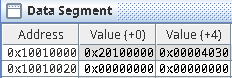
\includegraphics[width=.4\linewidth]{img/c1-10}
    \caption{Valores de las palabras en memoria correspondientes al vector de \mintinline{mips}{.byte}, tras indicar que los datos se almacenen desde la posición \texttt{0x10010002}}
    \label{fig:bytes-shift-endian}
\end{figure}

Teniendo esto en cuenta, vemos que los valores del vector de \mintinline{mips}{.byte} fueron almacenados en orden creciente respecto a posiciones de memoria que también crecen. Así, como en el programa indicamos los números \texttt{0x10}, \texttt{0x20}, \texttt{0x30} y \texttt{0x40} (en este orden), el primero de todos, el \texttt{0x10}, se encuentra en la posición de memoria \texttt{0x10010000}, luego el \texttt{0x20} en la posición \texttt{0x10010001}, y así sucesivamente.

Por ende, leemos el vector completo como el valor de una palabra \texttt{0x40302010} (siendo 4 elementos, exactamente la misma cantidad como hay de bytes en una palabra, siendo una sola suficiente para representar la totalidad de dicho vector). Mientras, guardar el valor \texttt{0x10203040} nos da una la pauta de cómo se hubieran almacenado los valores del vector en cuestión si el ensamblador hubiera tenido un comportamiento que se acercara a \textit{Big-Endian} (en el cual los ``últimos números'' se guardarían en las posiciones de memoria más pequeñas/bajas).

\subsection*{1.11}

A pesar del comportamiento de juntar los valores del tamaño de 1 byte en palabras, esto no afecta sobre los valores de las etiquetas \texttt{palabra1} y \texttt{palabra2}, que indican la primera posición de memoria desde la cual parte cada valor (en este caso, digamos, el vector y el segundo valor). Además, ayuda que puntualmente el vector definido en la consigna pueda estar contenido en una sola palabra, como ya mencionamos.

Por lo tanto, las etiquetas \texttt{palabra1} y \texttt{palabra2} toman los valores \texttt{0x10010000} y \texttt{0x10010004} respectivamente.

\begin{center}
\large\textbf{-- \textsl{Declaración de cadenas de caracteres} --}
\end{center}

\subsection*{1.12}

Para localizar la cadena ingresada en el programa dentro de la memoria, sabemos que debería de comenzar en la posición \texttt{0x10010000} ya que, como venimos repitiendo, es la dirección por defecto donde comienzan los datos si no se le provee un argumento a la directiva \mintinline{mips}{.data}.

Observando la valor de la palabra en la dirección mencionada, nos encontramos con el valor \textbf{\texttt{0x64636261}}. El patrón que tiene este valor es familiar con el explorado en la sección interior, en el cual veíamos cómo múltiples bytes estaban almacenados dentro de una palabra. Con esto en cuenta, podemos pensar que ésta posiblemente contenga los bytes individuales \texttt{0x61}, \texttt{0x62}, \texttt{0x63} y \texttt{0x64}, leyendo de posiciones menores a mayores en memoria. Considerando que la forma en que estos valores crecen se asemeja mucho con cómo nuestra cadena contiene caracteres consecutivos y lexicográficamente crecientes, sumado a que el nombre de la directiva utilizada en el programa para almacenar la cadena recibe el nombre de \mintinline{mips}{.ascii}, es intuitivo pensar que los bytes antes identificados se correspondan con las letras de la cadena en cuestión.

Comprobando nuestras sospechas, \texttt{0x61} equivale al número \texttt{97} en decimal, número correspondiente a la letra \texttt{\textquotesingle{}a\textquotesingle{}} en el código ASCII. Sucesivamente el resto de bytes equivalen en decimal entonces a los números \texttt{98}, \texttt{99} y \texttt{100}, correspondientes a las letras \texttt{\textquotesingle{}b\textquotesingle{}}, \texttt{\textquotesingle{}c\textquotesingle{}} y \texttt{\textquotesingle{}d\textquotesingle{}} en ASCII.

\begin{figure}[h]
    \centering
    \captionsetup{justification = centering}
    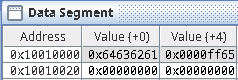
\includegraphics[width=.4\linewidth]{img/c1-12}
    \caption{Valores en memoria tras el ensamblado del código indicado}
    \label{fig:ascii-mem}
\end{figure}

De todas formas, debemos recordar que nuestra cadena era \texttt{\char34{}abcde\char34}, por lo que nos estaría faltando ubicar la letra \texttt{\textquotesingle{}e\textquotesingle{}}. Como podemos ver en la Figura \ref{fig:ascii-mem}, la próxima palabra en la posición \texttt{0x10010004} contiene el valor \textbf{\texttt{0x0000ff65}}. El \textsl{\texttt{65}} en las posiciones menos significativas del valor surge como continuación de la cadena de caracteres, el cual se encuentra en la posición de memoria siguiente al \textsl{\texttt{64}} de la palabra anterior, pero que se nos muestra de esta forma al tener que ubicarse por fuera del espacio de la primera palabra (en simples palabras, ``no entraba'' en la primera palabra), y por lo ya discutido en la sección anterior.

Luego, el \textsl{\texttt{ff}} que le sigue al \textsl{\texttt{65}} se corresponde con el valor almacenado con la directiva \mintinline{mips}{.byte} dentro del programa.

\subsection*{1.13}

Si empleamos la directiva \mintinline{mips}{.asciiz} en vez de la directiva \mintinline{mips}{.ascii} en el programa de la Cuestión anterior, el cambio que se observa es el agregado de lo que sería el equivalente a un byte \textit{vacío} entre el final de la cadena, y el próximo valor almacenado con la directiva \mintinline{mips}{.byte}. Es decir, mientras la primera palabra no cambia, la segunda en memoria toma ahora el valor \textbf{\texttt{0x00ff0065}}.

Este compartamiento es similar a la forma en la que, en lenguajes de programación como \texttt{C}, se agrega un caracter con valor ASCII = 0 al final de una cadena, conocido como el \textit{terminador} (generalmente representado como {\usemintedstyle{default}\mintinline{mips}{'\0'}}). Haciendo uso de este caracter, se puede determinar en qué punto finaliza una cadena de caracteres, incluso conociendo sólo el comienzo de la misma y que sus elementos se encuentran en posiciones de memroia consecutivas. Por lo tanto, al operar con ella, es sólo cuestión de recorrer todas estas posiciones partiendo desde la primera, hasta encontrarse con un byte \texttt{0x00} que indica el final.

\subsection*{1.14}

Podemos reemplazar la directiva \mintinline{mips}{.ascii} con la \mintinline{mips}{.byte} cargando posiciones en memoria con un vector de los caracteres de la cadena original, representados con su valor ASCII:

\vspace{7pt}
\inputminted[linenos]{mips}{src/cuestiones/c1-14.asm}
\vspace{7pt}

De hecho, podemos incluso utilizar los caracteres como tales, en vez de sus equivalentes en ASCII, y el ensamblador se encargará de transformarlos en sus valores numéricos correspondientes:

\vspace{7pt}
\inputminted[linenos]{mips}{src/cuestiones/c1-14b.asm}
\vspace{7pt}

\begin{center}
\large\textbf{-- \textsl{Reserva de espacio en memoria} --}
\end{center}

\subsection*{1.15 y 1.16}

Observando el panel de datos con los valores en la memoria (Fig. \ref{fig:space-mem}), podemos ver que se ha reservado el tamaño equivalente a exactamente dos palabras, para la variable \texttt{espacio}. Esto equivale a 8 bytes, entendiéndose así que el parámetro de la directiva \mintinline{mips}{.space} está expresado en cantidad de bytes que se quiere reservar en memoria.

Dicho esto, entonces el rango de posiciones que se han reservado en la memoria para la variable es [\texttt{\textbf{0x10010004}}, \texttt{\textbf{0x1001000b}}]. Las palabras en posiciones \texttt{0x10010000} y \texttt{0x1001000c} contienen los valores \texttt{0x20} y \texttt{0x30} respectivamente, declarados con la directiva \mintinline{mips}{.word} en el programa.

\begin{figure}[H]
    \centering
    \captionsetup{justification = centering}
    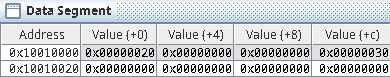
\includegraphics[width=.6\linewidth]{img/c1-15}
    \caption{Valores en memoria tras ensamblar el programa dado}
    \label{fig:space-mem}
\end{figure}

\begin{center}
\large\textbf{-- \textsl{Alineación de datos en memoria} --}
\end{center}

\subsection*{1.17}

Se reservó el rango de posiciones [\texttt{\textbf{0x10010001}}, \texttt{\textbf{0x10010004}}] en memoria para la variable \texttt{espacio}.

\subsection*{1.18}
\label{sec:c1-18}

Si bien los cuatro bytes reservados podrían contener la información de una palabra, éstos no podrían funcionar como tal ya que, como dijimos en la \hyperref[sec:c1-6]{Cuestión 1.6}, la memoria de una palabra tiene que \textit{estar alineada}, en el sentido que cada una debe comenzar en una posición de memoria múltiplo de 4.

Desde lo visto en la teoría, la arquitectura de MIPS nos permite leer información de la memoria de a una palabra a la vez, pues su tamaño equivale al ancho del bus de datos, y esto necesariamente debe ser en posiciones iniciales múltiplos de 4. Por tal motivo, si quisiérmos usar los 4 bytes reservados para \texttt{espacio} como un único espacio de memoria del tamaño de una palabra, realmente deberíamos acceder para cada operación necesaria a las palabras en las direcciones \texttt{0x10010000} y \texttt{0x10010004}, que lo hace poco práctico e ineficiente para este propósito. Esto sin mencionar las operaciones adicionales que se requerirían para juntar ambas palabras, o también descartar información en otras posiciones que se encuentren en las palabras, pero que no corresponda al espacio asignado para la tarea.

\subsection*{1.19}

El \texttt{byte1}, al haberse declarado al comienzo del programa, fue inicializado en la posición de memoria \textbf{\texttt{0x10010000}}. Mientras, como el \texttt{byte2} fue declarado al final del programa, éste fue posicionado en la dirección de memoria \textbf{\texttt{0x10010005}}, después del espacio reservado para la variable \texttt{espacio}.

\subsection*{1.20}

Finalmente, la variable \texttt{palabra} fue inicializada partiendo de la posición \texttt{\textbf{0x10010008}} en la memoria. Esto se debe a que como la variable fue declarada con la directiva \mintinline{mips}{.word}, ésta debe de ocupar una palabra entera, a pesar de que la memoria esté ocupada hasta la posición \texttt{0x10010005}. En consecuencia, la variable se ubica en la posición ya mencionada, teniendo en cuenta que la anterior palabra en la posición \texttt{0x10010004} tiene un byte ocupado por la variable \texttt{byte2}.

Esta situación es similar a la vista en la \hyperref[sec:c1-6]{Cuestión 1.6}, en el cual la declaración de una variable con \mintinline{mips}{.word} fue dada a partir del comienzo de la \textit{palabra} más próxima libre, en vez de comenzar desde la primera \textit{posición} libre.

\begin{figure}[H]
    \centering
    \captionsetup{justification = centering}
    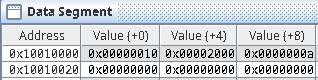
\includegraphics[width=.5\linewidth]{img/c1-17}
    \caption{Vista de la memoria posterior al emsamblado del código de las Cuestiones 1.17-1.20}
\end{figure}

\subsection*{1.21 y 1.22}

De haber entendido correctamente el rol de la directiva \mintinline{mips}{.align}, ésta hará que la próxima directiva de declaración de algún dato se coloque partiendo desde la próxima potencia de $2^n$, siendo n el argumento que recibe la directiva. En este caso, como la directiva recibe al número \textit{2} como argumento, la variable \texttt{espacio} se reservará partiendo desde la primera posición múltiplo de $2^2 = 4$ libre más cercana. Considerando que la primera posición de memoria libre a este punto es la \texttt{0x10010001} (ya que \texttt{byte1} ocupa la anterior), la próxima posición múltiplo de 4 disponible es la \texttt{0x10010004}. Podemos confirmar nuestra sospecha al ver el valor de la posición de memoria a la que hace referencia \texttt{espacio} en la ventana Labels (Fig. \ref{fig:c1-21-labels}).

\begin{figure}[h]
    \centering
    \captionsetup{justification = centering}
    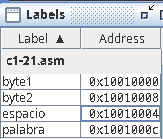
\includegraphics[width=.25\linewidth]{img/c1-21}
    \caption{Valores en memoria de las etiquetas para el código de las Cuestiones 1.21-1.22}
    \label{fig:c1-21-labels}
\end{figure}

Luego, como la directiva \mintinline{mips}{.space} recibe un \textit{4} como argumento, se reservan 4 posiciones desde la inicial, efectivamente inicializándose en el rango [\texttt{\textbf{0x10010004}}, \texttt{\textbf{0x10010007}}].

El hecho de reservar 4 posiciones de memoria (4 bytes), como también haber alineado la variable con una posición múltiplo de 4, hacen que el espacio reservado pueda constituir una palabra. No sólo el tamaño es igual al de una palabra (como ya vimos en la pregunta de la \hyperref[sec:c1-18]{Cuestión 1.18}), sino que también está alineada apropiadamente con el comienzo de una palabra. Al fin y al cabo, justamente es la directiva \mintinline{mips}{.align} la cual se encargó de hacerlo, ya que al indicarle el \textit{2} como argumento, alineó el espacio con una posición múltiplo de $2^2 = 4$, como es apropiado para una palabra (según lo discutido en la Cuestión mencionada).

Con todo esto en cuenta, podemos decir resumidamente que:

\begin{center}
    \textit{La directiva \mintinline{mips}{.align} ubica en memoria el próximo dato declarado a partir de la primera posición libre que sea múltiplo de $2^n$, siendo \textbf{n} el argumento pasado a la directiva.}
\end{center}

\section{Apartado 2}

\begin{center}
\large\textbf{-- \textsl{Carga de datos inmediatos (constantes)} --}
\end{center}

\subsection*{2.1}
\label{sec:c2-1}

La dirección de memoria donde se encuentra la instrucción en cuestión es la \texttt{\textbf{0x00400000}}, y ocupa el tamaño de exactamente una palabra (4 bytes = 32 bits). El valor que la representa es \texttt{0x3c108690}. Como sabemos que es una traducción de código en Assembly que conocemos, podemos deducir las partes que lo componen. Sin embargo, si bien algunas de ellas pueden ser reconocidas desde su representación en hexadecimal, deberemos de remitirnos a su equivalente en binario para darle completo sentido a cómo es que realmente funciona.

\begin{figure}[H]
    \centering
    \captionsetup{justification = centering}
    \texttt{\textbf{0\tikzmark{hex-lui-pref}x \textcolor{Red}{3c\tikzmark{hex-lui-tobin}10} \textcolor{Emerald}{86\tikzmark{hex-lui-ivalue}90}}}
    \begin{tikzpicture}[overlay, remember picture]
        \draw ($ (pic cs:hex-lui-pref) + (0,-.1) $) -- ($ (pic cs:hex-lui-pref) + (0,-.4) $) -| ($ (pic cs:hex-lui-pref) + (-3,-.6) $) node (pref) [label={[yshift=5pt]-90:\small{}\sffamily{}prefijo hexadecimal}] {};
        \draw ($ (pic cs:hex-lui-ivalue) + (0,-.1) $) -- ($ (pic cs:hex-lui-ivalue) + (0,-.4) $) -| ($ (pic cs:hex-lui-ivalue) + (3,-.6) $) node (ivalue) [label={[yshift=5pt]-90:\small{}\textcolor{Emerald}{\sffamily{}dato inmediato}}] {};

        \draw[-stealth] ($ (pic cs:hex-lui-tobin) + (0,-.1) $) -- ($ (pic cs:hex-lui-tobin) + (0,-.5) $) node (hex-tobin) [label={[yshift=2pt]-90:\textbf{\texttt{\textcolor{NavyBlue}{001\tikzmark{hex-lui-opcode}111}00\;000\textcolor{Purple}{10\tikzmark{hex-lui-reg}000}}}}] {};
        \draw ($ (hex-tobin) + (-.95,-.5) $) -- ($ (hex-tobin) + (-.95,-.7) $) -| ($ (hex-tobin) + (-2,-.9) $) node [label={[yshift=5pt]-90:\small\sffamily{}\textcolor{NavyBlue}{código de instrucción}}] {};
        \draw ($ (hex-tobin) + (1.075,-.5) $) -- ($ (hex-tobin) + (1.075,-.7) $) -| ($ (hex-tobin) + (2,-.9) $) node [label={[yshift=5pt]-90:\small\sffamily{}\textcolor{Purple}{número de registro}}] {};
    \end{tikzpicture}
    \vspace{50pt}
    \caption{Formato del valor contenido en memoria para la instrucción ingresada}
    \label{fig:lui-mem-hex}
\end{figure}

En la Figura \ref{fig:lui-mem-hex} vemos las 4 partes del valor en memoria para la instrucción:

\begin{itemize}
    \item El \textbf{prefijo hexadecimal}, el cual ya bien sabemos nos indica que un valor dado está representado en una notación numérica con base 16.
    \item El \textbf{código de instrucción} (conocido como \textit{opcode}), es decir, un valor que nos indica qué tipo de instrucción se está indicando a ejecutarse. En el código tratado, se corresponde con informar que se quiere llevar a cabo la instrucción \mintinline{mips}{lui}.

        El motivo por el cual para poder separar este campo debemos convertir en binario los primeros dos bytes de la palabra, es que el código de instrucción ocupa los primeros \textit{6} bits de la palabra. Por lo tanto, al pasarse a base 16, no es claramente distinguible. Por la misma razón así sucede con los siguientes dos grupos de 5 bits (el primero de ellos ignorado para la instrucción \mintinline{mips}{lui}).
    \item El \textbf{número de registro}, que contiene el identificador del registro al cual el dato inmediato será cargado. Si bien en código Assembly éste es representado con un nombre \mintinline{mips}{$s0}, internamente los registros son enumerados del 0 al 31, haciendo que esta abstracción sea interpretada por el ensamblador al cargarse la instrucción en memoria. De hecho, en el programa dado se puede reemplazar \mintinline{mips}{$s0} por \mintinline{mips}{$16} sin repercusiones.
    \item El \textbf{dato inmediato}, el cual como ya vimos en la teoría, es un valor del tamaño de media palabra (2 bytes = 16 bits), el cual será cargado en los 16 bits más significativos del registro especificado. Debido a su tamaño en bits múltiplo de 4, sumado a que se lo representa en el código en hexadecimal dentro del código en cuestión, lo hace fácil de distinguir en la representación en hexa del valor en memoria.
\end{itemize}

\subsection*{2.2}

Efectivamente, al correr el programa, los primeros 2 bytes del registro son cargados con el valor \texttt{0x8690}, así quedando la palabra almacenada en el registro como \textbf{\texttt{0x86900000}}.

\subsection*{2.3 y 2.4}
\label{sec:c2-4}

De forma similar a la Cuestión anterior, el dato inmediato especificado como argumento a la instrucción \mintinline{mips}{li} es cargado en el registro indicado como argumento. La diferencia es que este valor es del tamaño de una palabra completa, en vez de media palabra como sucedía con la instrucción \mintinline{mips}{lui}.

Ante esto, tras revisar la interpretación del código ensamblado en el panel de texto (\textit{Text Segment}), vemos que, siendo que \mintinline{mips}{li} es realmente una \textit{pseudoinstrucción}, fue descompuesta en dos instrucciones del procesador: la ya vista \mintinline{mips}{lui}, y otra llamada \mintinline{mips}{ori}. \vspace{7pt}

Conociendo ya el funcionamiento de \mintinline{mips}{lui} en base a lo visto en la Cuestión anterior, podemos entender que carga los primeros dos bytes (es decir, los más significativos) del valor inmediato utilizado en el código, al registro \mintinline{mips}{$at} (abreviación de \textit{Assembler Temporary}). Este registro está reservado por el ensamblador para las operaciones realizadas como \textit{pseudo comandos}, es decir, operaciones intermedias llevadas a cabo por las instrucciones reales que fueron obtenidas de la interpretación de una instrucción en el código Assembly.\footnote{\url{https://en.wikibooks.org/wiki/MIPS_Assembly/Register_File}} La interpretación de pseudoinstrucciones suele involucrar el uso del registro \mintinline{mips}{$at}, como es el caso en cuestión.


Posteriormente, se hace uso de la instrucción \mintinline{mips}{ori}, también llamada \textit{OR Immediate}, el cual dado un registro de destino, un registro origen y un valor inmediato, almacena el resultado de la operación \texttt{OR} binaria entre los últimos dos, en el registro de destino. El valor inmediato dicho debe de tener un tamaño de, al igual que en \mintinline{mips}{lui}, media palabra. Por lo tanto, en este caso, al correr esta instrucción se procede a almacenar en el registro de destino, originalmente especificado en la pseudoinstrucción \mintinline{mips}{li}, el resultado de hacer el \texttt{OR} binario entre:

\begin{itemize}
    \itemsep0em
    \item Los dos bytes menos significativos del valor que se quería cargar originalmente al registro en el programa.
    \item Los otros dos bytes anteriormente almacenados en \mintinline{mips}{$at} con la instrucción real \mintinline{mips}{lui}.
\end{itemize}

Notar que, como la instrucción \mintinline{mips}{lui} establece los otros dos bytes menos significativos de \mintinline{mips}{$at} en 0, aplicar a continuación la operación \texttt{OR} no afectará al valor inmediato con el que se opera, resultando en lo que podría considerarse como ``la carga de un valor'' para estos dos bytes.

\begin{figure}[h]
    \centering
    \captionsetup{justification = centering}
    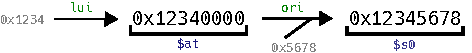
\includegraphics[width=.6\linewidth]{img/c2-4.pdf}
    \caption{\mintinline{mips}{li $s0, 0x12345678}, con las instrucciones reales que lo implementan}
\end{figure}

Pensando más a fondo, resulta claro el motivo de tener una pseudoinstrucción tal como \mintinline{mips}{li}. Y es que, con un tamaño de palabra de 32 bits, donde los registros pueden almacenar una palabra,  y las posiciones de memoria son accesibles por palabra, las instrucciones están limitadas a un máximo de 32 bits cada una. Como es estrictamente necesario que algunos de estos bits estén dedicados a indicar de qué instrucción se trata, es imposible disponer de los 32 bits que se quieran cargar sobre un registro, dentro de una sola instrucción. En consecuencia, la idea de una pseudoinstrucción que haga el trabajo de partir un valor inmediato proporcionado para que pueda ser cargado en un registro, ayuda a la legibilidad del código y facilita la tarea del programador.


\begin{center}
\large\textbf{-- \textsl{Carga de palabras (palabras de memoria a registro)} --}
\end{center}

\subsection*{2.5 y 2.6}
\label{sec:c2-6}

Como ya hemos dicho, la zona de memoria dedicada a instrucciones comienza a partir de la dirección \texttt{0x00400000}. Allí encontramos que el programa ensamblado ocupa 3 palabras, es decir, la única instrucción en el código después de la directiva \mintinline{mips}{.text} fue descompuesta por el ensamblador en tres instrucciones reales. Podemos ver cuáles son y los valores con los que son representados en memoria desde el panel de segmento de texto (Figura \ref{fig:c2-5}).

\begin{figure}[H]
    \centering
    \captionsetup{justification = centering}
    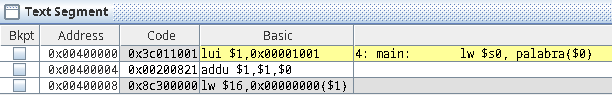
\includegraphics[width=.9\linewidth]{img/c2-5.png}
    \caption{Direcciones de memoria, instrucciones y sus valores en memoria, posteriores al ensamblado del programa dado}
    \label{fig:c2-5}
\end{figure}

Es curioso ver por qué el simulador tradujo la instrucción original en las 3 vistas en la figura anterior. Particularmente porque la instrucción \mintinline{mips}{lw} \textbf{no} es una pseudoinstrucción, sin mencionar que la última de las mencionadas 3 \textit{es una instrucción }\textsl{\mintinline{mips}{lw}}.

Debemos de recordar que la etiqueta \texttt{palabra} apunta a una dirección de memoria, por lo que tiene una longitud de 32 bits. Ya vimos en la sección anterior que es imposible contener un valor de tamaño tal en una sola instrucción, y es justamente por esto que el simulador recurre a un par de instrucciones adicionales para traducir la instrucción en el programa, a código máquina.

De esta forma, vemos en la primera instrucción traducida, el comienzo de un mecanismo muy similar al visto en la traducción de la pseudoinstrucción \mintinline{mips}{li}, donde los 2 bytes más significativos del valor inmediato son cargados en el registro temporal \mintinline{mips}{$at} mediante la instrucción \mintinline{mips}{lui}. Sin embargo, en contraste con el proceso visto en la Cuestión anterior, no se hace uso de la instrucción \mintinline{mips}{ori}.

La segunda de las instrucciones traducidas añade el valor del registro ingresado \mintinline{mips}{$0} (que ya sabemos siempre contendrá un cero) a los dos bytes más altos de \texttt{palabra} cargados en \mintinline{mips}{$at}, pareciendo ignorar los dos bytes menos significativos de \texttt{palabra}. Así luego, la tercera instrucción traducida utiliza como destino al registro así indicado en la instrucción original (\mintinline{mips}{$s0}), y el registro \mintinline{mips}{$at} junto con un valor inmediato \texttt{0x00000000} como dirección de memoria desde la cual cargar, permitiendo usar directamente el valor en \mintinline{mips}{$at} sin modificarlo.

A pesar de la omisión mencionada, como la dirección de \texttt{palabra} en este caso tiene sus dos bytes menos significativos en 0, el código ensamblado funciona correctamente. Por este motivo, podemos probar agregar en el código la declaración de una palabra adicional antes de \texttt{palabra}, que obligue a esta última a ubicarse en una posición de memoria donde sus dos bytes menos significativos sean distintos de cero:

\vspace{7pt}
\inputminted[linenos]{mips}{src/cuestiones/c2-6.asm}
\vspace{7pt}

Tras ensamblar el código con esta modificación, si bien no vemos instrucciones adicionales que consideren los dos bytes que creíamos eran omitidos, resulta que éstos son contemplados a partir del valor inmediato de la tercera instrucción traducida \mintinline{mips}{lw}. Como ésta admite una media palabra como valor inmediato, puede contener aquellos bytes menos significativos y sumárselos a los otros dos más significativos cargados en \mintinline{mips}{$at}, efectivamente representando la dirección de memoria de \texttt{palabra}, cuyo valor quiere cargarse en el registro \mintinline{mips}{$s0}.

Es por esto que vemos en el panel del segmento de texto, que el valor inmediato de \mintinline{mips}{lw} es \texttt{0x00000004}, para contar por el desfase de bytes que tuvo la etiqueta \texttt{palabra} tras agregar la declaración de una variable con la directiva \mintinline{mips}{.word} al comienzo del segmento de datos (\mintinline{mips}{.data}) [Fig. \ref{fig:c2-6}].

\begin{figure}[H]
    \centering
    \captionsetup{justification = centering}
    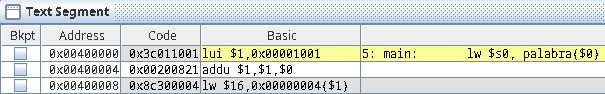
\includegraphics[width=.9\linewidth]{img/c2-6.png}
    \caption{Panel del segmento de texto tras introducir la declaración de una nueva variable del largo de una palabra, anterior a la declaración de \texttt{palabra}}
    \label{fig:c2-6}
\end{figure}

\subsection*{2.7}
\label{sec:c2-7}

\begin{itemize}
    \usemintedstyle{murphy}
    \item \mintinline{mips}{lui $1, 0x00001001} $\rightarrow$ \texttt{0x3c011001} = \texttt{\textcolor{murphy-green-pyg}{001111}00 000\textcolor{murphy-periwinkle-pyg}{00001} \textcolor{murphy-deepsea-pyg}{00010000 00000001}}
    \begin{itemize}
        \item \mintinline{mips}{lui} es la instrucción, su opcode es \texttt{0xF}, abarca los primeros 6 bits.
        \item \mintinline{mips}{$1} es el registro de destino, abarca 5 bits.
        \item \mintinline{mips}{0x00001001} o acortado \mintinline{mips}{0x1001} es un valor inmediato con una longitud de media palabra (últimos 16 bits).
    \end{itemize}

    La instrucción carga en los 16 bits más significativos del registro identificado como \mintinline{mips}{$1}, el valor inmediato \mintinline{mips}{0x1001}.

    \usemintedstyle{default}
    \item \texttt{\textcolor{murphy-green-pyg}{addu} \textcolor{cyan}{\$1}, \textcolor{magenta}{\$1}, \textcolor{Fuchsia}{\$0}} $\rightarrow$ \texttt{0x00200821} = \texttt{\textcolor{murphy-green-pyg}{000000}\textcolor{magenta}{00 001}\textcolor{Fuchsia}{00000} \textcolor{cyan}{00001}000 00\hl{100001}}
    \begin{itemize}
        \item \texttt{\textcolor{murphy-green-pyg}{addu}} es la instrucción, abarca los primeros 6 bits y comparte un opcode \texttt{0x0} con otras instrucciones.
        
        Se identifica de otras instrucciones con dicho opcode a partir de los bits en el campo conocido como \textit{funct}, que en este caso es \texttt{0x21}, y está arriba \hl{resaltado en amarillo}.

        \item \texttt{\textcolor{cyan}{\$1}} es el registro de destino, abarca 5 bits.
        \item \texttt{\textcolor{magenta}{\$1}} y \texttt{\textcolor{Fuchsia}{\$0}} son ambos registros de origen y operandos de la instrucción, abarcan 5 bits cada uno.
    \end{itemize}

    La instrucción escribe en el registro de destino \textcolor{cyan}{\texttt{\$1}}, el resultado de la suma \textit{no signada} (es decir, sin importar el signo) de los números almacenados en los registros de origen \texttt{\textcolor{magenta}{\$1}} y \texttt{\textcolor{Fuchsia}{\$0}}. Sabiendo que \texttt{\textcolor{Fuchsia}{\$0}} siempre contiene el número cero, y que el otro de los registros de origen es el mismo que el registro de destino, entonces el valor no cambia.

\item \texttt{\textcolor{murphy-green-pyg}{lw} \textcolor{cyan}{\$16}, \textcolor{magenta}{0x00000000}(\textcolor{Fuchsia}{\$1})} $\rightarrow$ \texttt{0x8c300000} = \texttt{\textcolor{murphy-green-pyg}{100011}\textcolor{Fuchsia}{00 001}\textcolor{cyan}{10000} \textcolor{magenta}{00000000 00000000}}
    \begin{itemize}
        \item \texttt{\textcolor{murphy-green-pyg}{lw}} es la instrucción, su opcode es \texttt{0x23}, abarca los primeros 6 bits.
        \item \texttt{\textcolor{cyan}{\$16}} es el registro de destino, abarca 5 bits.
        \item \texttt{\textcolor{magenta}{0x00000000}} o acortado \texttt{\textcolor{magenta}{0x0000}} es un valor inmediato con una longitud de media palabra (últimos 16 bits).
        \item \texttt{\textcolor{Fuchsia}{\$1}} es la dirección de un registro cuyo valor debe apuntar a una dirección de memoria (a la que luego se le sumará el valor inmediato en concepto de \textit{offset}). Abarca 5 bits.
    \end{itemize}

    La instrucción carga en el registro de destino \texttt{\textcolor{cyan}{\$16}} (también conocido como \mintinline{mips}{$s0}), el valor contenido en la dirección de memoria obtenida de la suma entre: el valor contenido en el registro \texttt{\textcolor{Fuchsia}{\$1}}, y el valor inmediato proporcionado \texttt{\textcolor{magenta}{0x0000}}.
\end{itemize}

\subsection*{2.8}

Como es de esperarse, al correr el programa, como \texttt{palabra} apunta a la dirección de memoria \texttt{0x10010000}, y el registro \mintinline{mips}{$0} siempre contiene un valor 0; se carga el valor contenido en la dirección \texttt{0x10010000} (o sea, directamente a la que apunta \texttt{palabra}), \texttt{\textbf{0x10203040}}, en el registro de destino \mintinline{mips}{$s0}.

\subsection*{2.9}

Para poder cargar la dirección de un dato en un registro, podemos usar la pseudoinstrucción \mintinline{mips}{la}. De esta forma podemos modificar el programa del ejercicio de manera que haga uso de dicha pseudoinstrucción, pero cumpliendo la misma tarea que el código original:

\vspace{7pt}
\inputminted[linenos]{mips}{src/cuestiones/c2-9.asm}
\vspace{7pt}

Verificando el panel del segmento de texto, podemos ver que la pseudoinstrucción utilizada, de forma prácticamente idéntica a la instrucción \mintinline{mips}{li} vista en las Cuestiones \hyperref[sec:c2-1]{2.1}-\hyperref[sec:c2-4]{2.4}, fue sustituida por las instrucciones \mintinline{mips}{lui} y \mintinline{mips}{ori}. Éstos son utilizados por el programa ensamblado para poder cargar los 2 bytes más significativos, y los 2 menos significativos, en el registro \mintinline{mips}{$t0}, respectivamente.

Como un comentario adicional, mencionar que hacemos uso del registro \mintinline{mips}{$t0} para almacenar la dirección de memoria a la que apunta la etiqueta \texttt{palabra}, ya que los registros comenzados en \textit{t} son generalmente utilizados para almacenar valores temporales. Es por esto la letra con la que comienzan: son \textit{\textbf{t}emporary}.

\subsection*{2.10}

Partiendo del programa ya modificado de la Cuestión anterior, modificarlo nuevamente para cargar en el registro \mintinline{mips}{$s0} la palabra que se encuentra desde \texttt{palabra+1} es tan sencillo como cambiar el valor inmediato de la instrucción \mintinline{mips}{lw}:

\vspace{7pt}
\inputminted[linenos]{mips}{src/cuestiones/c2-10.asm}
\vspace{7pt}

Ahora, en vez de usar el valor \mintinline{mips}{0x0000}, usamos el número \mintinline{mips}{1}, para desfasar la dirección \texttt{+1} posiciones. Así vemos que también podemos usar valores decimales como valor inmediato de la instrucción \mintinline{mips}{lw}.

Dicho esto, al intentar correr el programa, nos encontramos con un error de ejecución en la consola del simulador (Fig. \ref{fig:error-exec-2-10}).

\begin{figure}[H]
    \centering
    \captionsetup{justification = centering}
    \begin{tcolorbox}[fontupper=\small, width=.8\linewidth]
        \begin{Verbatim}[breaklines, breakanywhere, breaksymbol=, breakanywheresymbolpre=, commandchars=\\\{\}]
Error in \textbf{[\textit{redacted}]}/c2-10.asm line 5: Runtime exception at 0x00400008: fetch address not aligned on word boundary 0x10010001

Go: execution terminated with errors.
        \end{Verbatim}
    \end{tcolorbox}
    \caption{Error en la consola del simulador al intentar correr el código modificado}
    \label{fig:error-exec-2-10}
\end{figure}

Resulta que, como venimos insistiendo a lo largo del trabajo, las palabras en la memoria deben estar necesariamente alineadas con direcciones múltiplos de 4. Esto no excluye el acceso a la memoria, por lo que, sabiendo que \texttt{palabra} sí es una dirección de memoria válida, la dirección de memoria \texttt{palabra+1} resulta inválida al no ser múltiplo de 4 (considerando obvio que la dirección de memoria debe ser la del \textbf{primer} byte de la palabra). Debemos de entender que al sumarle un \texttt{1} a la dirección, a partir de cambiar el valor inmediato de la instrucción \mintinline{mips}{lw}, ésto la avanza en una posición, que se corresponde con un byte; no cuatro. 

De hecho, el error nos indica cuál es la dirección de memoria que produjo el error: \textbf{\texttt{0x10010001}}. Si el valor al que apunta \texttt{palabra} es el primero (y único) declarado en el segmento de datos, por defecto su dirección será \texttt{0x10010000}. Fácilmente se puede ver que \texttt{0x10010000} + 1 = \texttt{0x10010001}.

\subsection*{2.11}
\label{sec:c2-11}

Finalmente, para poder guardar los dos bytes de mayor peso (los más significativos) de \texttt{palabra} en \mintinline{mips}{$s0}, podemos ajustar el offset del valor inmediato de la instrucción \mintinline{mips}{lh} en \textit{2} posiciones respecto a la posición de \texttt{palabra}.

Esto funciona ya que al especificar una dirección, como estamos indicando que se cargue una media palabra, la operación será aplicada sobre el byte en la posición utilizada como argumento y la siguiente a ella; son 2 bytes. Por lo tanto, considerando lo explorado en la Cuestión \hyperref[sec:c1-10]{1.10}, sabiendo que MIPS (o al menos el simulador utilizado) almacena los valores bajo el formato \textit{Little-Endian}, implicaría que si utilizamos \texttt{palabra+2} como parámetro a \mintinline{mips}{lh}, los dos bits más significativos de la palabra serían cargados en el registro.

Recordar que \textit{Little-Endian} es un formato/orden donde los bits menos significativos se ubican en las posiciones de memoria más bajas. En este sentido, si no desfásaramos la posición de memoria de \texttt{palabra}, se tomarían los dos bits \textit{menos} significativos. Pues si la palabra comienza en la posición apuntada por la etiqueta, como ésta es la posición de memoria más baja entre las 4 que abarca, bajo el concepto de Little-Endian, resultaría que las primeras dos posiciones se corresponden con los bits de menor peso.

El código resultante es el siguiente:

\vspace{7pt}
\inputminted[linenos]{mips}{src/cuestiones/c2-11.asm}
\vspace{7pt}

Llama la atención que al tratarse de medias palabras, no hay fallos del simulador en cuanto a que la dirección especificada no sea múltiplo de 4. Al parecer, con \textit{halfwords}, las direcciones deben estar alineadas con múltiplos de 2, ya que si intentamos reemplazar la instrucción [\mintinline[escapeinside=||]{mips}{lh $s0, |\hl{2}|($t0)}] con \mintinline[escapeinside=||]{mips}{lh $s0, |\hl{3}|($t0)}, el simulador falla al ejecutar el programa de una forma muy similar a la vista en la Figura \ref{fig:error-exec-2-10}. La única diferencia es que el mensaje advierte sobre el \texttt{halfword boundary} en vez del \texttt{word boundary}.


\begin{center}
\large\textbf{-- \textsl{Carga de bytes (bytes de memoria a registro)} --}
\end{center}

\subsection*{2.12}

Al ensamblar el programa, vemos que la instrucción \mintinline{mips}{lb} es traducida en memoria de instrucciones de forma muy similar a cómo lo hemos visto con la instrucción \mintinline{mips}{lw} en la Cuestión \hyperref[sec:c2-6]{2.6}. Como ya vimos, el Assembler lleva a cabo este procedimiento debido a la incapacidad de poder especificar directamente direcciones de memoria completas en una sola instrucción. Po ello, debe recurrir a un procedimiento análogo al mencionado en la anterior Cuestión:

\begin{enumerate}
    \item Cargar los 2 bytes más significativos de la dirección de memoria a la que apunta, en este caso \texttt{octeto}, al registro temporal \mintinline{mips}{$at}. [Instrucción \mintinline{mips}{lui}]
    \item Añadir el valor del registro especificado en conjunto con el valor inmediato (\mintinline{mips}{$0} para este caso), al valor en \mintinline{mips}{$at}. [Instrucción \mintinline{mips}{addu}]
    \item Reformular la instrucción \mintinline{mips}{lb} sumando el registro \mintinline{mips}{$at} a un valor inmediato que contiene los dos bits menos significativos de \texttt{octeto}.
\end{enumerate}

Es decir, en resumen, si bien \mintinline{mips}{lb} carga el byte de una dirección de memoria en un registro, la forma de especificar la dirección, como es para nuestro ejemplo con la etiqueta \texttt{octeto}, no cambia el hecho que su longitud sea de 32 bits, y que por ello deba de cargarse como ya hemos visto, por las limitaciones de la longitud de los registros de instrucciones.

\begin{figure}[H]
    \centering
    \captionsetup{justification = centering}
    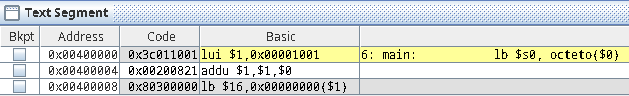
\includegraphics[width=.9\linewidth]{img/c2-12.png}
    \caption{Instrucciones traducidas por el simulador tras ensamblar el programa dado}
\end{figure}

\subsection*{2.13 y 2.14}
\label{sec:c2-14}

Al ejecutar el programa, nos encontramos con un compartamiento un poco diferente al esperado. Lo que probablemente creíamos que sucedería es que, tal y como nos fue dicho en la teoría, que el byte en la dirección de memoria \texttt{octeto} se cargue en el registro \mintinline{mips}{$s0}. Sin embargo, el valor que termina cargándose en dicho registro, es \textbf{\texttt{0xfffffff3}}.

Ante la disyuntiva propuesta luego en la Cuestión 2.14, probamos ejecutar el programa tras cambiar la instrucción \mintinline{mips}{lb} por \mintinline{mips}{lbu}. Efectivamente, al correr el programa con este cambio, sí produce el efecto esperado. Ahora se carga el valor \textbf{\texttt{0x000000f3}} en el registro.

La pregunta entonces es, ¿cuál es la diferencia entre \mintinline{mips}{lb} y \mintinline{mips}{lbu}? ¿qué significa esa \texttt{u} al final?

\begin{figure}[h]
    \centering
    \captionsetup{justification = centering}
    \begin{tabular}{l l r c l}
        \texttt{octeto} y \mintinline{mips}{$s0} (\mintinline{mips}{lbu}) & $\rightarrow$ & \texttt{0xf3} &=& \texttt{00000000 00000000 00000000 11110011} \\
        \mintinline{mips}{$s0} (\mintinline{mips}{lb}) & $\rightarrow$ & \texttt{0xfffffff3} &=& \texttt{11111111 11111111 11111111 11110011}
    \end{tabular}

    \caption{Representaciones binarias de los números con los que trabajamos}
    \label{fig:bin-2-14}
\end{figure}

Curiosamente, ya hemos visto la \texttt{u} mencionada al final de una instrucción: en \mintinline{mips}{addu}. Para entender mejor esto, veamos las representaciones binarias de los números tratados (Fig. \ref{fig:bin-2-14}).

Como podemos ver, la única diferencia entre ambos números es el estado de los bits en los primeros tres bytes de mayor peso: con \mintinline{mips}{lb} son todos establecidos en 1, mientras que se mantienen en 0 con \mintinline{mips}{lbu}.

Consultando en documentación de MIPS, resulta que dicha \texttt{u} proviene de \textit{\textbf{u}nsigned}. Nos estábamos saltando por alto la forma en la que la computadora interpretaba internamente los números.

Según hemos visto con LC-3, necesariamente los números deben estar representados en código binario para poder ser almacenados en la memoria. Por lo tanto, si bien en el simulador vemos su representación hexadecimal (o decimal, cambiando una opción), no podemos simplemente asumir que los números se van a sumar mágicamente como estamos acostumbrados.

Con esto en cuenta, debemos comprender que en el caso de MIPS, los números son representados como complemento a 2 (\textit{2's complement}), y soporta operaciones tanto con números \texttt{signed} como \texttt{unsigned}. Nos referimos a que con los números \texttt{signed}, podemos representar números negativos, con el costo de poder representar poco menos de la mitad de números positivos (concretamente, $2^{31} - 1$ positivos, pero también $2^{31}$ negativos, y el 0). Así, cuando una instrucción que lleve a cabo operaciones aritméticas o que maneje números en memoria, no tenga una letra \texttt{u} al final de su nombre, se entiende que tratará los valores proporcionados como enteros signados.

Volviendo entonces a la diferencia entre el comportamiento de \mintinline{mips}{lb} y \mintinline{mips}{lbu}, podemos entender cómo \mintinline{mips}{lb}, al ver que el bit más significativo en el byte al que apunta \texttt{octeto} es un 1 (indicando que es negativo), al ser cargado en un registro con una longitud del cuádruple del valor dicho, extiende aquel \textit{1} hacia todos los bits nuevos en el registro \mintinline{mips}{$s0}, con el fin de \textbf{mantener el signo} del número original.

En cambio, como \mintinline{mips}{lbu} trata los números como enteros sin signo, ignora este detalle, y carga el valor en el registro, dejando el resto de bits en 0.

\subsection*{2.15}

Si se cambia la definición de \texttt{octeto} para ahora apuntar a un byte cuyo valor sea \texttt{0x30}, no existe diferencia entre el uso de \mintinline{mips}{lb} y \mintinline{mips}{lbu}. Esto se debe a que si observamos la representación binaria de \texttt{0x30} (\texttt{00110000}), el estado del bit más significativo es 0, indicando que como entero signado, es positivo. Por consecuencia, si usamos \mintinline{mips}{lb}, para mantener el signo establecerá los bits restantes en \mintinline{mips}{$s0} en 0. Mientras, como \mintinline{mips}{lbu} ya por defecto deja el resto de bits en 0, el efecto de ambas instrucciones es el mismo.

\subsection*{2.16}

Definiendo ahora a \texttt{octeto} para apuntar al valor de una palabra cuyo valor sea \texttt{0x10203040}, el valor cargado en \mintinline{mips}{$s0} es \textbf{\texttt{0x00000040}}.

El motivo de esto es similar al visto en la Cuestión \hyperref[sec:c2-11]{2.11} usando la instrucción \mintinline{mips}{lb} para cargar bytes, en vez de \mintinline{mips}{lh} para medias palabras. Cuando \mintinline{mips}{lb} recibe la dirección de memoria del comienzo de la palabra a la que apunta \texttt{octeto}, la instrucción interpretará cargar en el registro el byte que se encuentra en esa dirección. Sabiendo que el simulador almacena los valores en memoria bajo el formato \textit{Little-Endian}, el valor de este byte será entonces el de los 4 bits menos significativos de la palabra en \texttt{octeto}, el cual en este caso es \texttt{0x40}.

Además, el hecho considerar el número como signado mediante el uso de \mintinline{mips}{lb} no afecta a los bits restantes en el registro, pues el estado del bit más significativo en \texttt{0x40} es 0.

\subsection*{2.17}

Cambiando la instrucción en \texttt{main} para cargar en el registro el valor en \texttt{octeto+1}, en vez de \texttt{octeto}, resulta en que el valor en \mintinline{mips}{$s0} sea \textbf{\texttt{0x00000020}} tras ejecutar el programa.

En este caso no se produce error alguno, a diferencia de cómo si habíamos visto que sucedía con la instrucción \mintinline{mips}{lw} para cargar palabras, por ejemplo. La razón de esto es que en este caso estamos cargando \textit{bytes}, por lo que cualquier direccción de memoria es válida para un byte. El concepto de que ``la memoria esté alineada'' con múltiplos de 4 no aplica para bytes, ya que con las palabras, éstas tienen una longitud de 4 bytes, mientras las variables declaradas como \mintinline{mips}{.byte}, bueno, ocupan un byte. En todo caso, la regla consistiría en que las direcciones de memoria ``estén alineadas con múltiplos de 1'', lo cual abarca a todas las direcciones de memoria posibles.

La idea de que la memoria esté alineada está directamente relacionada con la longitud del campo con el que tratamos. Con \textit{palabras} es con múltiplos de 4 por sus 4 bytes de longitud, con \textit{medias palabras} es con múltiplos de 2 por sus 2 bytes de longitud, y con los \textit{bytes} es con múltiplos de 1 por su único 1 byte de longitud.

En lo que concierne al motivo del valor cargado en \mintinline{mips}{$s0}, estamos viendo el efecto de haber cargado el valor al que apunta la etiqueta \texttt{siguiente}. Como \texttt{octeto} apunta a un \mintinline{mips}{.byte}, según lo ya visto en el apartado de \textsl{\hyperref[sec:decl-byte-mem]{declaración de bytes en memoria}}, como la siguiente variable declarada (\texttt{siguiente}) también es del tipo \mintinline{mips}{.byte}, éste se ubica en la posición de memoria inmediatamente siguiente a la de \texttt{octeto}. Por lo tanto, la dirección a la que apunta \texttt{octeto+1}, es efectivamente la misma a la que apunta \texttt{siguiente}, la cual contiene el byte \texttt{0x20} que fue cargado en \mintinline{mips}{$s0}.

Comentar también que como el estado del bit más significativo en \texttt{0x20} es 0, no se presentan diferencias que partan del uso de \mintinline{mips}{lb} para cargar este valor en el registro \mintinline{mips}{$s0}.


\begin{center}
    \large\textbf{-- \textsl{Almacenado de palabras (palabras de registro a memoria)} --}
\end{center}

\subsection*{2.18}
\label{sec:c2-18}

La primera instrucción del programa es \mintinline{mips}{lw}, la cual ya hemos visto y mencionado reitaradas veces en este trabajo. En consecuencia, su traducción por parte del simulador es idéntica a la descripta y analizada en la Cuestión \hyperref[sec:c2-7]{2.7}. Ver la Figura \ref{fig:c2-18} por el detalle de este caso concreto.

\begin{figure}[H]
    \centering
    \captionsetup{justification = centering}
    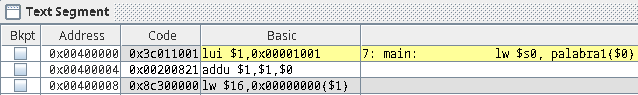
\includegraphics[width=.9\linewidth]{img/c2-18}
    \caption{Traducción del simulador de la primera instrucción del programa provisto}
    \label{fig:c2-18}
\end{figure}

\subsection*{2.19}

Para poder comprobar mejor el efecto de la ejecución del programa, comparemos lado a lado el estado de la memoria antes y después de ejecutarlo (Fig. \ref{fig:side-by-side-2-19}).

\begin{figure}[H]
    \centering
    \captionsetup{justification = centering}
    \subfloat[Estado antes de ejecutar el programa]{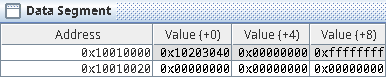
\includegraphics[width=.6\linewidth]{img/c2-19a}}\\
    \subfloat[Estado después de ejecutar el programa]{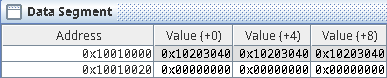
\includegraphics[width=.6\linewidth]{img/c2-19b}}
    \caption{Comparación del estado de los valores de la memoria, antes y después de ejecutar el programa}
    \label{fig:side-by-side-2-19}
\end{figure}

Antes de ejecutar el programa, están cargados 3 valores en memoria, cada una ocupando el espacio de una palabra. En orden: \texttt{0x10203040}, \texttt{0x00000000} y \texttt{0xffffffff}.

Tras ejecutar el programa, las tres palabras contienen el mismo valor: \textbf{\texttt{0x10203040}}.

Si vemos el paso a paso de las instrucciones del programa, podemos entender el motivo de esto:

\begingroup
\setlength{\emergencystretch}{3em}
\begin{enumerate}
    \item La instrucción \mintinline{mips}{lw} carga la palabra en la dirección de memoria marcada con la etiqueta \texttt{palabra1}, \textbf{\texttt{0x10203040}}, en el registro \mintinline{mips}{$s0}.
    \item Luego, la instrucción \mintinline{mips}{sw} \textbf{escribe} el valor en el registro \mintinline{mips}{$s0}, \textbf{\texttt{0x10203040}}, en la dirección de memoria a la que apunta \texttt{palabra2} (recordar que no agregamos offset porque el registro de operando es \mintinline{mips}{$0}, que siempre contiene el valor 0), \textbf{reemplazando} el valor anteriormente allí almacenado, \textsl{\texttt{0x00000000}}.
    \item Finalmente, de forma similar a la anterior instrucción, \mintinline{mips}{sw} \textbf{escribe} el valor de \mintinline{mips}{$s0} (\textbf{\texttt{0x10203040}})  en la dirección de memoria a la que apunta la etiqueta \texttt{palabra3}, \textbf{reemplazando} el valor anteriormente allí almacenado \texttt{0xffffffff}.
\end{enumerate}
\endgroup

En conclusión, el programa sobreescribe el valor en las palabras a las que apuntan las etiquetas \texttt{palabra2} y \texttt{palabra3}, con el valor en la palabra a la que apunta \texttt{palabra1}.

\begin{center}
    \large\textbf{-- \textsl{Almacenado de bytes (bytes de registro a memoria)} --}
\end{center}

\subsection*{2.20}

Al igual que en la Cuestión \hyperref[sec:c2-18]{2.18}, la primera instrucción es \mintinline{mips}{lw}, por lo que ya sabemos cómo es traducida por el simulador.

En cuanto a la instrucción \mintinline{mips}{sw}, su traducción es similar a la de \mintinline{mips}{sw}, donde la forma en la que se carga la dirección de memoria a la que apunta \texttt{octeto} se corresponde con la ya descripta en la Cuestión \hyperref[sec:c2-6]{2.6}, con la diferencia de que la tercera instrucción es \mintinline{mips}{sb} en vez de \mintinline{mips}{lw}, pues es la instrucción que tradujo el simulador.

\begin{figure}[H]
    \centering
    \captionsetup{justification = centering}
    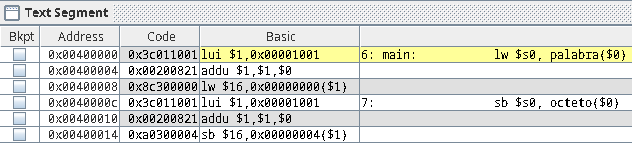
\includegraphics[width=.9\linewidth]{img/c2-20}
    \caption{Traducción de las instrucciones del programa por el simulador}
\end{figure}

\subsection*{2.21}

Antes de ejecutar el programa, \texttt{octeto} apunta a un espacio en memoria del tamaño de media palabra.

Luego de correrlo, la instrucción \mintinline{mips}{lw} carga la palabra a la que apunta \texttt{palabra} (\texttt{0x10203040}), en el registro \mintinline{mips}{$s0}. Posteriormente, aquel valor es utilizado por la instrucción \mintinline{mips}{sb} para escribir el byte \textbf{menos significativo} de la palabra, en la dirección de memoria a la que apunta \texttt{octeto}. Como dijimos que el valor es \texttt{0x10203040}, su byte menos significativo se encuentra en la primera posición de memoria de la palabra (por la naturaleza \textit{Little-Endian} del simulador), así éste byte siendo \textbf{\texttt{0x40}}.

En consecuencia, \texttt{octeto} guarda el valor \textbf{\texttt{0x0040}}, el cual expresamos como media palabra pues ésta es la longitud del espacio a la que apunta la etiqueta.

\subsection*{2.22}

Para lograr el cambio pedido, podemos cambiar la instrucción [\mintinline{mips}{sb $s0, octeto($0)}], por [\mintinline[breaklines]{mips}{sb $s0, octeto+1($0)}]. Producto de este cambio, ahora \texttt{octeto} contiene el valor \textbf{\texttt{0x4000}} tras ejecutar el programa.

Antes, al usar \texttt{octeto} directamente, se apuntaba al byte menos significativo del espacio al que la etiqueta apuntaba, por el formato \textit{Little-Endian}. Al desfasar la dirección de memoria por un byte (reemplzando \texttt{octeto} por \texttt{octeto+1}), ahora el byte menos significativo de la palabra almacenada en \mintinline{mips}{$s0} (allí cargada por la instrucción previa \mintinline{mips}{lw}), se escribe mediante el uso de \mintinline{mips}{sb} en el segundo byte menos significativo de \texttt{octeto} (que siendo el caso de una media palabra, es directamente la posición de mayor peso).

Es por este motivo que ahora \texttt{octeto} toma el valor \texttt{0x4000}, y en el código original \texttt{0x0040}: vemos el desfase de un byte de la posición a la que \mintinline{mips}{sb} escribe.

\subsection*{2.23}

Notar que como el programa original utiliza la instrucción \mintinline{mips}{lw} para cargar la palabra \textbf{entera} en el registro \mintinline{mips}{$s0}, y luego \mintinline{mips}{sb} toma el byte menos significativo de allí para escribirlo en octeto, \textbf{no podemos} simplemente cambiar \texttt{palabra} por \texttt{palabra+3} en la instrucción \mintinline{mips}{lw}. La instrucción \mintinline{mips}{lw} requiere la posición de una palabra, entonces tiene que ser múltiplo de 4, a lo que \texttt{palabra+3} no cumple esta condición.

Por lo tanto, para lograr la consigna pedida, podemos cambiar la instrucción \mintinline{mips}{lw} por \mintinline{mips}{lbu}, la cual ya vimos en la Cuestión \hyperref[sec:c2-14]{2.14}. De esta forma, ahora sí podemos reemplazar \texttt{palabra} por \texttt{palabra+3}, cargando desde un principio el byte ubicado en \texttt{palabra+3}, al registro \mintinline{mips}{$s0}. Luego la instrucción \mintinline{mips}{sb} tomará el byte en el registro, y lo escribirá en la posición de menor peso del espacio al cual apunta \texttt{octeto}.

El código resultante es el siguiente:

\vspace{7pt}
\inputminted[linenos]{mips}{src/cuestiones/c2-23.asm}
\vspace{7pt}

Aclarar que hacemos uso de la instrucción \mintinline{mips}{lbu} en vez de \mintinline{mips}{lb}, para evitar cualquier diferencia que pueda surgir de interpretar el byte como un número signado. Si bien, en teoría, en este caso no debería hacer la diferencia dado que el bit menos significativo de \texttt{0x10} no está prendido, usamos \mintinline{mips}{lbu} para más generalidad.

\section{Apartado 3}

\begin{center}
    \large\textbf{-- \textsl{Operaciones aritméticas con datos inmediatos (constantes)} --}
\end{center}

\subsection*{3.1}

El resultado de la suma efectuada se alamacena en el registro \mintinline{mips}{$t1}. Se suma 1 al valor de la palabra a la que apunta la etiqueta \texttt{numero}, el cual corresponde al máximo número positivo representable \texttt{0x7fffffff}. Por consiguiente, el valor contenido en \mintinline{mips}{$t1} tras ejecutar el programa es \textbf{\texttt{0x80000000}}.

\subsection*{3.2 y 3.3}
\label{sec:c3-3}

Al intentar correr el programa después de cambiar la instrucción \mintinline{mips}{addiu} por \mintinline{mips}{addi}, vemos que la ejecución falla informándonos el motivo el origen del error en la consola (Fig. \ref{fig:error-overflow}).

\begin{figure}[H]
    \centering
    \captionsetup{justification = centering}
    \begin{tcolorbox}[fontupper=\small, width=.8\linewidth]
        \begin{Verbatim}[breaklines, breakanywhere, breaksymbol=, breakanywheresymbolpre=, commandchars=\\\{\}]
Error in \textbf{[\textit{redacted}]}/c3-2.asm line 6: Runtime exception at 0x0040000c: arithmetic overflow

Step: execution terminated with errors.
        \end{Verbatim}
    \end{tcolorbox}
    \caption{Error en la consola del simulador al intentar correr el código tras cambiar la instrucción \mintinline{mips}{addiu} por \mintinline{mips}{addi}}
    \label{fig:error-overflow}
\end{figure}

A partir de haber corrido el programa paso a paso, y como también se menciona en el error devuelto por consola, el problema surge en la línea 6 del programa. La causa es advertida como \textit{arithmetic overflow}. Es decir, al sumarle un número positivo (valor inmediato igual a 1) al ya máximo número entero positivo representable (contenido en la palabra a la que apunta la etiqueta \texttt{numero}), el resultado se excede del límite representable, resultando en una excepción de desbordamiento (\textit{overflow}).

Precisamente ésta es la diferencia entre las instrucciones \mintinline{mips}{addi} y \mintinline{mips}{addiu}: ambas permiten sumar un valor inmediato a un registro, pero con la diferencia en que la variante \textbf{no} terminada en \textit{u}, provoca una excepción en el caso de producirse una instancia de \textit{overflow} al llevar a cabo la operación aritmética.

\begin{center}
    \large\textbf{-- \textsl{Operaciones aritméticas con datos en memoria} --}
\end{center}

\subsection*{3.4 y 3.5}

El programa en cuestión obtiene el resultado de la resta de los valores a los que apuntan las etiquetas: \texttt{numero1} $-$ \texttt{numero2} $-$ \texttt{numero3}. Esta diferencia se almacena en la palabra a la que apunta \texttt{numero1} al final del programa (\textbf{NO} en \texttt{numero3}, como sugiere el enunciado), mediante la instrucción \mintinline{mips}{sw}.

En este caso, el resultado almacenado en dicha dirección es \textbf{\texttt{0x7ffffffe}}. Sin embargo, considerando que los números con los que operamos están representados como enteros signados, el valor obtenido es \textbf{incorrecto}. Considerando que \texttt{0x80000000} es el mínimo número negativo representable (en decimal, $-2147483648$), restarle 2 ($-1-1$, concretamente) si bien no falla al usar la instrucción \mintinline{mips}{subu}, resulta en un valor que ``salta'' al otro lado de la recta numérica, resultando en un valor correspondiente a un número positivo (en decimal, $2147483646$).

Es por esta situación de desbordamiento que hay diferencia al usar la instrucción \mintinline{mips}{sub} en vez de \mintinline{mips}{subu}. Sustituyendo las instrucciones de esta manera, el programa falla en la línea 9 al ejecutarlo a paso, con un error idéntico al visto en la Figura \ref{fig:error-overflow}. La única diferencia con lo visto en la Cuestión \hyperref[sec:c3-3]{3.3}, es que en este caso el error se produce por sobrepasar el límite del \textit{mínimo número entero signado representable}, en vez del límite del \textit{máximo entero signado representable}, como fue el caso de la Cuestión mencionada.

\begin{center}
    \large\textbf{-- \textsl{Multiplicación y división con datos en memoria} --}
\end{center}

\subsection*{3.6}

Después de realizar la operación, se obtiene el resultado de la multiplicación entre los valores contenidos en las palabras a las que apuntan las etiquetas \texttt{numero1} y \texttt{numero2}, es decir, \texttt{0x7fffffff} $\cdot$ 16.

Debido a que el producto entre los dos números en cuestión sobrepasa el límite representable de números positivos signados, la instrucción \mintinline{mips}{mult} permite prescindir del argumento que especifique el registro al que se almacene el resultado (en comparación con \mintinline{mips}{mul}), de forma que se almacene el resultado dividido en dos registros especiales: \mintinline{mips}{$hi} y \mintinline{mips}{$lo}.

Como pueden llegar a sugerir los nombres de estos registros, \mintinline{mips}{$hi} almacena los 4 bytes más significativos del resultado, mientras que \mintinline{mips}{$lo} almacena los 4 menos significativos. Para poder acceder a estos registros especiales, se requiere del uso de las instrucciones \mintinline{mips}{mfhi} y \mintinline{mips}{mflo} respectivamente, las cuales cargarán su valor en un registro especificado como argumento.

Así, para el código dado, el resultado es almacenado en las posiciones \texttt{0x10010008} y \texttt{0x1001000c}, que al concatenarlas nos da el valor \texttt{0x7fffffff0} (en decimal, 4611686014132420609), que como es de esperarse, representa correctamente el producto entre los factores aclarados en el primer párrafo.

Finalizando con una aclaración a lo explicado del resultado del producto, notar que nunca necesitaremos más de dos palabras para almacenarlo, siempre que los factores sean dos números almacenados cada uno en una palabra. Pues el producto más grande posible, \texttt{0x7fffffff} $\cdot$ \texttt{0x7fffffff} (o en decimal, $2147483647 \; \cdot \; 2147483647 = 2147483647^2$), da igual a \texttt{0x3fffffff00000001}, que es menor al mayor número representable con dos palabras (64 bits), \texttt{0x7fffffffffffffff}. {\emergencystretch3em\par}

\subsection*{3.7}

Podemos modificar de forma sencilla el código anterior para que divida el valor en \texttt{numero1} por el de \texttt{numero2}. Luego de cambiar los datos a los que apuntan las etiquetas dichas según lo indica el ejercicio, podemos cambiar la instrucción \mintinline{mips}{mult} por \mintinline{mips}{div}, la cual guarda el resto de la división en el registro especial \mintinline{mips}{$hi}, y el cociente en el registro especial \mintinline{mips}{$lo}.

Como ya leíamos los contenidos de estos registros y los escribíamos a continuación de los números en memoria (por usar \mintinline{mips}{mult} previamente), el único cambio restante es invertir las instrucciones \mintinline{mips}{mflo} y \mintinline{mips}{mfhi} de lugar, con el único propósito de almacenar primero el cociente, y luego el resto en memoria, según se da a entender en el enunciado.

El programa resultante es el siguiente:

\vspace{7pt}
\inputminted[linenos]{mips}{src/cuestiones/c3-7.asm}
\vspace{7pt}

\begin{center}
    \large\textbf{-- \textsl{Operaciones lógicas} --}
\end{center}

\subsection*{3.8}

Modificamos el código del enunciado para cumplir con la consigna, a partir de sustituir el valor inmediato usado en \mintinline{mips}{andi} por \textbf{\texttt{0xffff0001}}, ya que su representación en binario tiene los 16 bits más significativos y el bit 0 prendidos: \texttt{11111111 11111111 00000000 00000001}.

\vspace{7pt}
\inputminted[linenos]{mips}{src/cuestiones/c3-8.asm}
\vspace{7pt}

El valor almacenado en \texttt{numero+4} con estas modificaciones resulta \textbf{\texttt{0x00030001}}. Comparándolo con el valor original, cumple con la tarea solicitada.

\begin{figure}[H]
    \centering
    \captionsetup{justification = centering}
    \begin{tabular}{l l r c l}
        \texttt{numero} & $\rightarrow$ & \texttt{0x0003ff41} &=& \texttt{\textcolor{magenta}{00000000 00000011} \textcolor{gray}{11111111 0100000}\textcolor{magenta}{1}} \\
    \texttt{numero+4} & $\rightarrow$ & \texttt{0x00030001} &=& \texttt{\textcolor{magenta}{00000000 00000011} \textcolor{gray}{00000000 0000000}\textcolor{magenta}{1}}
    \end{tabular}

    \caption{Representaciones binarias de la palabra original y el resultado tras ejecutar el programa modificado}
    \label{fig:bin-3-8}
\end{figure}

\subsection*{3.9}

Como el ejercicio requiere que ciertos bits queden en 1 en vez de 0, no podemos cumplir con la consigna tan solo modificando la instrucción \mintinline{mips}{andi}. Como se describe en la teoría, este operador puede mantener bits si es que están establecidos en ambos operandos, o apagarlos si es que se encuentra en este estado en alguno de los dos números. Por lo tanto, como no podemos modifcar el valor en la palabra, aplicando la operación de \texttt{AND} binario con un valor inmediato solo podemos apagar o mantener bits ya prendidos en \texttt{numero}.

Para asegurarnos que los bits indicados siempre estén en 1 en el resultado, haremos uso de una instrucción adicional \mintinline{mips}{ori}, la cual aplica el \texttt{OR} binario entre un número en un registro y un valor inmediato. Esta operación mantiene un bit apagado si así se encuentra en \textbf{ambos} operandos, o permite encenderlo si el bit se encuentra en 1 en \textbf{alguno} de los dos números.

Como tenemos control sobre el valor inmediato, tras haber hecho la operación \texttt{AND} necesaria para mantener los bits pedidos por el ejercicio, luego usamos la instrucción \mintinline{mips}{ori} con la constante \texttt{0xfffe}. Este valor que usamos como valor inmediato, tiene todos los 16 bits menos significativos prendidos, a excepción del bit 0 (que debía de permanecer igual que en \texttt{numero} para el resultado), asegurándonos que dichos bits siempre estén en 1: \texttt{11111111 11111110}.

\vspace{7pt}
\inputminted[linenos]{mips}{src/cuestiones/c3-9.asm}
\vspace{7pt}

El valor resultante de la ejecución del programa es \textbf{\texttt{0x0003ffff}}. Comparándolo con el valor original, cumple con la tarea solicitada.

\begin{figure}[H]
    \centering
    \captionsetup{justification = centering}
    \begin{tabular}{l l r c l}
        \texttt{numero} & $\rightarrow$ & \texttt{0x0003ff41} &=& \texttt{\textcolor{magenta}{00000000 00000011} \textcolor{cyan}{11111111 0100000}\textcolor{magenta}{1}} \\
        \texttt{numero+4} & $\rightarrow$ & \texttt{0x0003ffff} &=& \texttt{\textcolor{magenta}{00000000 00000011} \textcolor{cyan}{11111111 1111111}\textcolor{magenta}{1}}
    \end{tabular}

    \caption{Representaciones binarias de la palabra original y el resultado tras ejecutar el programa modificado}
    \label{fig:bin-3-9}
\end{figure}

\begin{center}
    \large\textbf{-- \textsl{Operaciones de desplazamiento} --}
\end{center}

\subsection*{3.10, 3.11 y 3.14}
\label{sec:c3-11}

Vemos que a pesar de haber realizado una operación de desplazamiento de bits a la derecha, si bien los bits menos significativos correspondientes fueron descartados, los 4 bits más significativos fueron rellenados con el valor 1. En concreto, estos últimos bits fueron rellenados acorde al bit de signo (el más significativo), el cual está prendido para el caso del valor al que apunta \texttt{numero} en nuestro programa. El valor almacenado en \mintinline{mips}{$t1} tras ejecutar el programa es \texttt{0xfffffff4}.

Para entender mejor el motivo de esto, intentaremos ahora reemplazar la instrucción \mintinline{mips}{sra} por \mintinline{mips}{srl}. Ahora, al correr el programa, el valor guardado en el registro \mintinline{mips}{$t1} es \texttt{0x0ffffff4}. Es decir, con este cambio, los 4 bits más significativos \textbf{no} fueron rellenados con el bit de signo, y quedaron en 0.

Lo que está sucediendo se encuentra en la diferencia entre las dos instrucciones utilizadas. Por un lado, \mintinline{mips}{sra} lleva a cabo del desplazamiento \textit{\textbf{a}ritmético} de un número hacia la derecha, una cantidad de posiciones indicadas como argumento. Mientras, \mintinline{mips}{srl} ejecuta el desplzamiento \textit{\textbf{l}ógico} de un número, una cantidad de posiciones dada.

Con esto queremos decir que desde el punto de vista lógico, si desplazamos un número $n$ bits a la derecha, sabemos que los $n$ bits menos significativos serán descartados, y que el resto de bits se desplzarán de forma acorde, quedando las posiciones de los anteriores $n$ bits más significativos en 0, pues podemos decir que todo número tiene ``infinitos ceros'' a su izquierda. 

En cambio, si queremos desplazar un número una cantidad de posiciones desde el punto de vista aritmético, lo más probable es que sea de interés mantener el signo del número original. Como shifteamos bits en un sistema de representación binario, correrlos $n$ posiciones a la derecha es equivalente a dividir el número por $2^n$ y redondear el resultado para abajo (operación floor).

Considerando que al desplazar \texttt{numero} 4 posiciones a la derecha lo quisiéramos dividir por $2^4 = 16$, podemos terminar de cerrar la idea comparando las representaciones decimales de los números obtenidos con las instrucciones \mintinline{mips}{sra} y \mintinline{mips}{srl} (Fig. \ref{fig:bin-cmp-3-11}).

\begin{figure}[H]
    \centering
    \captionsetup{justification = centering}
    \begin{tabular}{l c c c l}
        \texttt{numero} &=& \texttt{0xffffff41} &=& $-191$ \\
        \mintinline{mips}{$t1} (\mintinline{mips}{sra}) &=& \texttt{0xfffffff4} &=& $-12$ = $\lfloor\frac{-191}{16}\rfloor$ \\
        \mintinline{mips}{$t1} (\mintinline{mips}{srl}) &=& \texttt{0x0ffffff4} &=& $268435444$
    \end{tabular}
    \caption{Diferencia en los resultados obtenidos entre desplazar \texttt{numero} con \mintinline{mips}{sra} y \mintinline{mips}{srl}}
    \label{fig:bin-cmp-3-11}
\end{figure}

\subsection*{3.12 y 3.13}
\label{sec:c3-13}

Para desplazar el contenido de \texttt{numero} 2 bits a la izquierda, reemplazamos la instrucción \mintinline{mips}{sra} por \mintinline{mips}{sll} y cambiamos el argumento de la cantidad de posiciones que se shiftea:

\vspace{7pt}
\inputminted[linenos]{mips}{src/cuestiones/c3-12.asm}
\vspace{7pt}

Si comparamos la representación decimal del número original con el del resultado obtenido (Fig. \ref{fig:bin-cmp-3-13}), podemos ver que acabamos de multiplicar el número por $2^n$, siendo $n = 2$ la cantidad de posiciones que desplazamos del número, o sea, $2^2 = 4$.

\begin{figure}[H]
    \centering
    \captionsetup{justification = centering}
    \begin{tabular}{l c c c l}
        \texttt{numero} &=& \texttt{0xffffff41} &=& $-191$ \\
        \mintinline{mips}{$t1} (\mintinline{mips}{sll}) &=& \texttt{0xfffffd04} &=& $-764$ = $-191 \cdot 2^2$ \\
    \end{tabular}
\caption{Diferencia entre el número original y el resultado obtenido usando \mintinline{mips}{sll}}
    \label{fig:bin-cmp-3-13}
\end{figure}

Notar que usamos la instrucción \mintinline{mips}{sll}, finalizada en \textit{l}, indicando que es una operación del tipo \textit{lógica}, y no \textit{aritmética} como distinguimos en la Cuestión \hyperref[sec:c3-11]{3.11}. Esto se debe a que \textbf{no existe} una instrucción tal como ``\texttt{sla}'', pues simplemente \textbf{no es necesaria}.

Recordemos que el inconveniente que surgía de usar el desplazamiento de bits lógico hacia la derecha, era que no se preservaba el bit de signo. En cambio, al realizar shifts hacia la izquierda, el signo se preserva. Si bien los bits más significativos en las $n$ posiciones de mayor peso son descartados (desplazando $n$ posiciones), los bits en las posiciones subsiguientes ocuparán su lugar manteniendo el signo según sea acorde.

Por supuesto, habrá un punto en el que, por ejemplo, si tenemos un número negativo, al desplazar bits exista la posibilidad de que quede un 0 en la posición del bit de signo, según cómo sea la representación binaria del número tratado. Pero ya para este punto, o incluso para varios shifts antes, el valor obtenido habría superado el límite representable por un número entero signado de 32 bits, requiriendo otro tipo de medidas para poder almacenar el resultado.

\chapter{Problemas}

\begin{center}
    \Large\textbf{-- Apartado 1 --}
\end{center}

\section{}

\usemintedstyle{autumn}
\inputminted[linenos]{mips}{src/problemas/1.asm}
\usemintedstyle{default}

En \textcolor{autumn-red-pyg}{\textbf{rojo}} se indican las etiquetas, en \textcolor{autumn-blue-pyg}{\textbf{azul}} las directivas, en \textcolor{autumn-gray-pyg}{\textbf{gris}} los comentarios, y en \textcolor{autumn-teal-pyg}{\textbf{celeste}} las instrucciones.

\section{}

\inputminted[linenos]{mips}{src/problemas/2.asm}

Utilizo dos directivas \mintinline{mips}{.space} pasándoles el número \textit{80} como argumento pues si una palabra son 4 bytes, y cada vector tiene que tener 20 palabras: $20 \cdot 4\;\text{bytes} = 80\;\text{bytes}$.

\section{}

\inputminted[linenos]{mips}{src/problemas/3.asm}


\section{}

\inputminted[linenos]{mips}{src/problemas/4.asm}


\section{}

\inputminted[linenos, breaklines, breakbytokenanywhere]{mips}{src/problemas/5.asm}


\section{}

\inputminted[linenos]{mips}{src/problemas/6.asm}

En ambos casos uso vectors de bytes, ya que los números de la matriz son lo suficientemente pequeños para ser almacenados de esta manera.

Al guardar la matriz por filas, termina resultando en un orden creciente, ya que entendemos que al ``almacenar por filas''. vamos guardando las filas de arriba hacia abajo, y los valores de cada una se almacenarán de forma consecutiva, como se leen de izquierda a derecha.

Mientras, al guardar la matriz por columnas, entendemos que almacenamos las columnas de izquierda a derecha, y que los valores de cada una de ellas se almacenarán de forma consecutiva, como se leen de arriba a abajo.

\begin{figure}[h]
    \centering
    \captionsetup{justification = centering}
    \subfloat[Almacenar por filas]{
        \begin{tabular}{!{\vrule width 1.5pt}c|c|c!{\vrule width 1.5pt}}
            \noalign{\hrule height 1.5pt}
            \rowcolor{LimeGreen!50}
            1 & 2 & 3 \\
            \noalign{\hrule height 1.5pt}
            \rowcolor{Violet!50}
            4 & 5 & 6 \\
            \noalign{\hrule height 1.5pt}
            \rowcolor{RoyalBlue!50}
            7 & 8 & 9 \\
            \noalign{\hrule height 1.5pt}
        \end{tabular}

        $\rightarrow$

        \begin{tabular}{!{\vrule width 1.5pt}>{\columncolor{LimeGreen!50}}c|>{\columncolor{LimeGreen!50}}c|>{\columncolor{LimeGreen!50}}c!{\vrule width 1.5pt}>{\columncolor{Violet!50}}c|>{\columncolor{Violet!50}}c|>{\columncolor{Violet!50}}c!{\vrule width 1.5pt}>{\columncolor{RoyalBlue!50}}c|>{\columncolor{RoyalBlue!50}}c|>{\columncolor{RoyalBlue!50}}c!{\vrule width 1.5pt}}
            \noalign{\hrule height 1.5pt}
            1 & 2 & 3 & 4 & 5 & 6 & 7 & 8 & 9 \\
            \noalign{\hrule height 1.5pt}
        \end{tabular}
    }


    \subfloat[Almacenar por columnas]{
        \begin{tabular}{!{\vrule width 1.5pt}>{\columncolor{LimeGreen!50}}c!{\vrule width 1.5pt}>{\columncolor{Violet!50}}c!{\vrule width 1.5pt}>{\columncolor{RoyalBlue!50}}c!{\vrule width 1.5pt}}
            \noalign{\hrule height 1.5pt}
            1 & 2 & 3 \\
            \hline
            4 & 5 & 6 \\
            \hline
            7 & 8 & 9 \\
            \noalign{\hrule height 1.5pt}
        \end{tabular}

        $\rightarrow$

        \begin{tabular}{!{\vrule width 1.5pt}>{\columncolor{LimeGreen!50}}c|>{\columncolor{LimeGreen!50}}c|>{\columncolor{LimeGreen!50}}c!{\vrule width 1.5pt}>{\columncolor{Violet!50}}c|>{\columncolor{Violet!50}}c|>{\columncolor{Violet!50}}c!{\vrule width 1.5pt}>{\columncolor{RoyalBlue!50}}c|>{\columncolor{RoyalBlue!50}}c|>{\columncolor{RoyalBlue!50}}c!{\vrule width 1.5pt}}
            \noalign{\hrule height 1.5pt}
            1 & 4 & 7 & 2 & 5 & 8 & 3 & 6 & 9 \\
            \noalign{\hrule height 1.5pt}
        \end{tabular}
    }
    \caption{Visualización de las dos formas de almacenar la matriz $A$ del ejercicio}
\end{figure}


\begin{center}
    \Large\textbf{-- Apartado 2 --}
\end{center}

\section{}

\inputminted[linenos]{mips}{src/problemas/7.asm}

Cabe mencionar que como los números del vector son menores al máximo número representable con una media palabra, podría definirse un vector de valores del tipo \mintinline{mips}{.half} en vez de \mintinline{mips}{.word}, acomodando las operaciones y desfases utilizados en el programa:

\inputminted[linenos]{mips}{src/problemas/7b.asm}

\section{}
\label{sec:p8}

Podemos extender el programa del ejercicio anterior y utilizar la instrucción \mintinline{mips}{sw} para cargar los valores que ya tenemos dentro de los registros \mintinline{mips}{$s0}-\mintinline{mips}{$s4}, en las palabras empezando desde la dirección \texttt{0x10010000}.

Además, podemos intentar optimizar la cantidad de instrucciones reales que usa nuestro programa, lo cual podría ayudar a la velocidad de nuestro programa. Por supuesto que con un programa tan pequeño, más aún corriendo en un simulador, no tiene mucho sentido optimizar la velocidad de ejecución del código. Sin embargo, resulta interesante explorar las distintas opciones y usos de las instrucciones ya vistas, para cumplir el objetivo del ejercicio.

\inputminted[linenos]{mips}{src/problemas/8.asm}

La idea fundamental de las optimizaciones realizadas, es evitar usar el uso de etiquetas o valores inmediatos muy grandes como parámetro a las instrucciones \mintinline{mips}{lw} o \mintinline{mips}{sw}, ahorrando las instrucciones adicionales que requiere cargar valores que superen la longitud de media palabra.

Para lograr esto, indicamos los offsets en el campo del valor inmediato (ya que son números chicos), y usamos el campo del registro que es sumando para determinar la dirección de memoria desde la cual leer/escribir, con un registro temporal que contenga como valor la dirección de memoria inicial con la cual estamos copiando. Es decir, si queremos leer valores desde las direcciones \texttt{V}, \texttt{V+2}, ..., cargamos la dirección de \texttt{V} una sola vez a un registro temporal, y luego usamos ese registro como parámetro para la instrucción \mintinline{mips}{lw}, mientras los valores inmediatos que se indican en las instrucciones son \texttt{1}, \texttt{2}, ...

\section{}

Una forma de resolver el problema planteado es cargando la palabra dada en un registro, y luego ir cargando en orden inverso, byte por byte en el espacio de la nueva palabra.

Para esto utilizaremos la instrucción \mintinline{mips}{lw} para cargar la palabra en \mintinline{mips}{$t1}, y luego la instrucción \mintinline{mips}{sb} para cargar los bytes en otro espacio de memoria. Como ésta última carga el byte menos significativo del registro, también usaremos la instrucción \mintinline{mips}{srl} que shiftea los bits hacia la derecha una cantidad de posiciones (concretamente 8 bits = 1 byte), descartando los bytes menos significativos una vez cargados en la nueva palabra, y corriendo de posición los más significativos a posiciones de menor peso para que podamos usar \mintinline{mips}{sb}.

\inputminted[linenos]{mips}{src/problemas/9.asm}

Como una alternativa, también podemos optar por una solución más rudimentaria, que aproveche la facilidad de cargar bytes desde una posición de memoria dada a un registro, y que luego los copie a otra posición de memoria en la palabra donde se almacenen los bytes en orden inverso. En este caso, podríamos prescindir del uso de la instrucción \mintinline{mips}{srl}, usando sólamente instrucciones vistas hasta este punto en el trabajo.

\inputminted[linenos]{mips}{src/problemas/9b.asm}

\section{}

\inputminted[linenos]{mips}{src/problemas/10.asm}

\section{}

Considerando que los 4 bytes se encuentran a partir de la dirección de memoria \texttt{0x10010002}, podemos resolver el problema con dos pares de operaciones de lectura y escritura de medias palabras usando \mintinline{mips}{lh} y \mintinline{mips}{sh} respectivamente:
\begin{itemize}
    \item Copiar desde [\texttt{0x10010002}, \texttt{0x10010003}] a [\texttt{0x10010010}, \texttt{0x10010011}].
    \item Copiar desde [\texttt{0x10010004}, \texttt{0x10010005}] a [\texttt{0x10010012}, \texttt{0x10010013}].
\end{itemize}

Además, cargamos las direcciones de memoria del vector almacenado y el espacio de memoria reservados con la instrucción \mintinline{mips}{la} en dos registros, para reducir la cantidad de operaciones según lo describimos en el \hyperref[sec:p8]{Problema 8}.

\inputminted[linenos]{mips}{src/problemas/11.asm}

\section{}

\inputminted[linenos]{mips}{src/problemas/12.asm}

\section{}

La opción más sencilla para resolver el ejercicio sería realizar la misma serie de pasos para cada número del vector:

\begin{itemize}
    \item Cargar el valor del vector en un registro.
    \item Realizar la división con el número 5 en un registro donde fue precargado.
    \item Leer el resultado del registro especial \mintinline{mips}{mflo}.
    \item Escribir el resultado en memoria.
\end{itemize}

\inputminted[linenos]{mips}{src/problemas/13a.asm}

También podemos explorar nuevos horizontes y usar branching consultando con la documentación:

\inputminted[linenos]{mips}{src/problemas/13b.asm}

Como siempre, probablemente existan otras formas más prácticas o más eficientes de realizar la tarea. Por ejemplo, seguramente se podría hacer uso de algún contador, en vez de comparar que la dirección de memoria de donde leemos el vector no pase de la posición del último número.

\section{}

Hacemos uso de la instrucción \mintinline{mips}{andi} con la constante \texttt{0xfffffd77} que tiene todos los bits menos el 3, 7 y 9, establecidos en 1, manteniendo así el resto de bits del entero original, y apagando los exceptuados:

\inputminted[linenos]{mips}{src/problemas/14.asm}

Tras ejecutar el programa, el entero en la memoria cambia al valor \textbf{\texttt{0xabcd1035}}. Comparando su representación binaria con la del número original, podemos ver cómo cumple con la consigna solicitada (Fig. \ref{fig:bin-cmp-14}).

\begin{figure}[H]
    \centering
    \captionsetup{justification = centering}
    \begin{tabular}{l c l}
        \texttt{0xabcd12bd} &=& \texttt{10101011 11001101 000100\textcolor{red}{1}0 \textcolor{red}{1}011\textcolor{red}{1}101} \\
        \texttt{0xabcd1035} &=& \texttt{10101011 11001101 000100\textcolor{red}{0}0 \textcolor{red}{0}011\textcolor{red}{0}101} \\[-3pt]
                            && \myrepeat{24}{\phantom{\texttt{0}}}{\scriptsize{}\;\!9}\myrepeat{2}{\phantom{\texttt{0}}}\;\!{\scriptsize{}7}\myrepeat{3}{\phantom{\texttt{0}}}\;\!{\scriptsize{}3}
    \end{tabular}
    \caption{Diferencia entre el número original y el modificado tras ejecutar el programa anterior usando la instrucción \mintinline{mips}{andi}}
    \label{fig:bin-cmp-14}
\end{figure}

\section{}

Interpretando que ``cambiar'' el valor de los bits del entero implica invertir su estado original, podemos usar la instrucción \mintinline{mips}{xori}, que hace el \texttt{XOR} binario con un valor inmediato dado. Utilizaremos la constante \texttt{0x288} para esta operación, ya que tiene los bits 3, 7 y 9 encendidos, de forma que puedan cambiarse en el número original.

\inputminted[linenos]{mips}{src/problemas/15.asm}

Después de correr el programa, el valor de la palabra es \textbf{\texttt{0xff0f10bd}}, el cual podemos comprobar que cumple con la consigna, comparando su representación binaria con la del número original (Fig. \ref{fig:bin-cmp-15}).


\begin{figure}[H]
    \centering
    \captionsetup{justification = centering}
    \begin{tabular}{l c l}
        \texttt{0xff0f1235} &=& \texttt{11111111 00001111 000100\textcolor{red}{1}0 \textcolor{red}{0}011\textcolor{red}{0}101} \\
        \texttt{0xff0f10bd} &=& \texttt{11111111 00001111 000100\textcolor{red}{0}0 \textcolor{red}{1}011\textcolor{red}{1}101} \\[-3pt]
                            && \myrepeat{24}{\phantom{\texttt{0}}}{\scriptsize{}\;\!9}\myrepeat{2}{\phantom{\texttt{0}}}\;\!{\scriptsize{}7}\myrepeat{3}{\phantom{\texttt{0}}}\;\!{\scriptsize{}3}
    \end{tabular}
    \caption{Diferencia entre el número original y el modificado tras ejecutar el programa anterior usando la instrucción \mintinline{mips}{xori}}
    \label{fig:bin-cmp-15}
\end{figure}

\section{}

Sabiendo que el número por el cual debemos multiplicar el dato almacenado en memoria, es una potencia de 2, podemos utilizar lo visto en la Cuestión \hyperref[sec:c3-13]{3.13} y usar la instrucción \mintinline{mips}{sll} shifteándolo 5 posiciones a la izquierda (pues $32 = 2^5$).

\inputminted[linenos]{mips}{src/problemas/16.asm}

Comparando las representaciones decimales del número original y el resultado obtenido, podemos confirmar que el programa anterior resuelve el problema propuesto (Fig. \ref{fig:bin-16}).

\begin{figure}[H]
    \centering
    \captionsetup{justification = centering}
    \begin{tabular}{c c l}
        \texttt{0x00001237} &=& $4663$ \\
        \texttt{0x000246e0} &=& $149216$ = $4663 \cdot 2^5$ \\
    \end{tabular}
    \caption{Diferencia entre el número original y el resultado obtenido usando \mintinline{mips}{sll}}
    \label{fig:bin-16}
\end{figure}


\end{document}
